%=================================================================
\documentclass[article,article,submit,pdftex,moreauthors]{Definitions/mdpi} 
%\documentclass[preprints,article,submit,pdftex,moreauthors]
% MDPI internal commands - do not modify
\firstpage{1} 
\makeatletter 
\setcounter{page}{\@firstpage} 
\makeatother
\pubvolume{1}
\issuenum{1}
\articlenumber{0}
\pubyear{2026}
\copyrightyear{2026}
%\externaleditor{Firstname Lastname} % More than 1 editor, please add `` and '' before the last editor name
\datereceived{ } 
\daterevised{ } % Comment out if no revised date
\dateaccepted{ } 
\datepublished{ } 
%\datecorrected{} % For corrected papers: "Corrected: XXX" date in the original paper.
%\dateretracted{} % For retracted papers: "Retracted: XXX" date in the original paper.
%\doinum{} % Used for some special journals, like molbank
%\pdfoutput=1 % Uncommented for upload to arXiv.org
%\CorrStatement{yes} % For updates
%\longauthorlist{yes} % For many authors that exceed the left citation part
%\IsAssociation{yes} % For association journals

%=================================================================
% Add packages and commands here. 
\usepackage{algorithmic}
\usepackage[export]{adjustbox}
\usepackage{textcomp}
\usepackage{lscape}
\usepackage{supertabular}
\usepackage{csquotes}
\usepackage{lipsum}
\usepackage{tabularray}
\usepackage{longtable}
\usepackage{amsfonts}
% \usepackage{changepage}

%=================================================================
% Please use the following mathematics environments: Theorem, Lemma, Corollary, Proposition, Characterization, Property, Problem, Example, ExamplesandDefinitions, Hypothesis, Remark, Definition, Notation, Assumption
%% For proofs, please use the proof environment (the amsthm package is loaded by the MDPI class).

%=================================================================
% Full title of the paper (Capitalized)
\Title{RLSFLoc: Reinforcement Learning-Based Adaptive Fusion for Fault Localization in Scalable Software Systems}

% Author Orchid ID: enter ID or remove command
\newcommand{\orcidauthorA}{0000-0000-0000-000X} % Add \orcidA{} behind the author's name
%\newcommand{\orcidauthorB}{0000-0000-0000-000X} % Add \orcidB{} behind the author's name

% Authors, for the paper (add full first names)
\Author{Muhammad Jamil $^{1,2}$, Sema Bayraktar $^{2}$, Alpaslan Burak \.{I}nner $^{1,2}$, Adnan Kavak $^{1,2}$, Muhammad Farhan $^{3}$, Gautam Srivastava $^{4,5}$ and Hossein Fotouhi $^{6}$*}

%\longauthorlist{yes}

% MDPI internal command: Authors, for metadata in PDF
\AuthorNames{Muhammad Jamil, Sema Bayraktar, Alpaslan Burak \.{I}nner, Adnan Kavak, Muhammad Farhan, Gautam Srivastava and Hossein Fotouhi}

% Affiliations / Addresses (Add [1] after \address if there is only one affiliation.)
\address{%
$^{1}$ \quad Department of Computer Engineering, Kocaeli University, Kocaeli 41001, Türkiye; jamil138.amin@gmail.com (M.J.); burak.inner@gmail.com(A.B.I.) akavak@kocaeli.edu.tr (A.K.)\\

$^{2}$ \quad Wireless Information and Intelligent Systems (WINS) Research Center, Kocaeli University, Kocaeli 41001, Türkiye; bayraktar.sema41@gmail.com (S.B.)\\

$^{3}$ \quad Department of Computer Science, COMSATS University Islamabad, Sahiwal Campus, 57000, Pakistan; farhansajid@gmail.com (M.F.)\\

$^{4}$ \quad Department of Computer Science and Engineering, 
Sogang University, Seoul 04107, Republic of Korea; gsrivast@ieee.org (G.S.) \\

$^{5}$ \quad Research Center for Interneural Computing, 
China Medical University, Taichung 40402, Taiwan \\

$^{6}$ \quad Department of Computer Science and Computer Engineering, Mälardalen University (MDU), 72123 Västerås, Sweden; hossein.fotouhi@mdu.se (H.F.)}

% Corresponding author
\corres{Correspondence: hossein.fotouhi@mdu.se (H.F.); gsrivast@ieee.org  (G.S.); akavak@kocaeli.edu.tr (A.K)}


\abstract{
Software fault localization plays an important role in reducing debugging effort and improving software maintenance. Traditional Spectrum-Based Fault Localization (SBFL) methods, such as Tarantula, Ochiai, and DStar, mainly depend on passed and failed test coverage and often fail to capture semantic meaning and structural dependency relationships among program elements. To address these limitations, this paper proposes \textbf{RLSFLoc}, a reinforcement learning-enhanced semantic and structural fault localization framework for scalable software fault localization. RLSFLoc integrates execution trace analysis, structural dependency graph propagation, semantic code representation, and reinforcement learning-based adaptive fusion to generate a ranked list of suspicious program elements. The proposed method formulates fault localization as a ranking-oriented decision-making problem, where the reinforcement learning agent learns adaptive fusion weights for execution, structural, and semantic evidence. The framework was evaluated using AEEEM \cite{dambros2010aeeem} and Defects4J \cite{just2014defects4j} under within-project and cross-project settings. The experimental results show that RLSFLoc achieves Top-1, Top-3, Top-5, and Top-10 accuracy values of 0.80, 1.00, 1.00, and 1.00, respectively, with an MRR of 0.8917, a MAP of 0.8917, and a mean EXAM score of 0.0230 (representing only 2.30\% of the codebase inspected). Compared with implemented spectrum-, learning-, graph-, and semantic-representation-based baselines, RLSFLoc improves early fault ranking while maintaining acceptable runtime and memory overhead. These results indicate that adaptive fusion of execution, semantic, and structural evidence can improve fault localization effectiveness and support practical debugging workflows in modern software engineering.
}

\keyword{
Software Fault Localization;
Reinforcement Learning;
Semantic Code Representation;
Structural Dependency Graph;
Spectrum-Based Fault Localization;
Debugging Automation
}
%%%%%%%%%%%%%%%%%%%%%%%%%%%%%%%%%%%%%%%%%%

\begin{document}

%%%%%%%%%%%%%%%%%%%%%%%%%%%%%%%%%%%%%%%%%%
\section{Introduction}
\label{sec:introduction}

Software systems are becoming increasingly large, interconnected, and difficult to maintain. Modern software projects often contain thousands of files, methods, classes, and execution paths. When a failure occurs, developers must identify the exact faulty program element responsible for the observed error. This process is commonly performed through manual debugging, code inspection, test analysis, and repeated execution. As software size and complexity increase, manual debugging becomes expensive, time-consuming, and error-prone. Therefore, automated fault localization has become an important research direction in software engineering because it helps developers identify suspicious code locations more efficiently \cite{wong2016survey,sarhan2022survey,wong2023overview,kochhar2016practitioners}. Fault localization aims to rank program elements according to their likelihood of being faulty. Traditional Spectrum-Based Fault Localization (SBFL) methods, such as Tarantula \cite{jones2005tarantula}, Ochiai \cite{abreu2007ochiai}, and DStar \cite{wong2014dstar}, use passed and failed test coverage to compute suspiciousness scores. These methods are simple, fast, and widely used. However, they mainly depend on execution spectra and cannot fully capture the semantic meaning of source code or the structural dependencies among program elements. As a result, they may produce weak rankings when several statements or methods have similar coverage patterns \cite{pearson2017evaluation,zhang2021pagerank,beszedes2022frequency}. Information Retrieval (IR)-based fault localization methods address this issue by using textual similarity between bug reports and source-code elements \cite{zhou2012buglocator,saha2013bluir,le2015better}. These methods can capture semantic relationships between failure descriptions and code identifiers, comments, or method names. However, their performance depends heavily on the quality of bug reports and naming conventions \cite{mills2020queries,kim2021trustworthy,chaparro2019query}. Similarly, neural representation approaches can learn richer code representations, but they often require training data and computational resources and require attention to interpretability \cite{li2019deepfl,lou2021grace,widyasari2022xai4fl}.

A major limitation in existing fault localization research is the gap between execution evidence, semantic evidence, and structural evidence. Execution evidence shows which program elements are involved in failed tests. Semantic evidence captures the meaning of code and bug descriptions. Structural evidence describes call relations, control-flow dependencies, data-flow links, and module-level interactions. Many existing methods use one principal evidence type or combine multiple evidence sources using learned or fixed strategies \cite{xuan2014learning,sohn2017fluccs,le2016ltr,lou2021grace,zeng2022smartfl,yan2023propagation}. However, the importance of each evidence source may change across different bugs, projects, and program contexts. Therefore, an adaptive fusion strategy is worth investigating for robust fault localization. To address this limitation, this paper proposes RLSFLoc, a reinforcement learning-enhanced semantic and structural fault localization framework for scalable software fault localization. RLSFLoc integrates execution trace analysis, structural dependency graph construction, semantic code representation, RL-based adaptive fusion, and a final fault ranking engine. The proposed framework first computes execution-based suspiciousness from passed and failed test cases. It then constructs a structural dependency graph to model relationships among program elements. In parallel, semantic representations are extracted from source code and bug-related textual information. These evidence sources are normalized and adaptively fused using a reinforcement learning agent that learns how much importance should be assigned to execution, structural, and semantic scores.

The motivation for using reinforcement learning is that fault localization can be formulated as a ranking-oriented decision-making problem. The goal is not only to classify whether a program element is faulty, but to rank faulty elements as high as possible so that developers can inspect fewer candidates \cite{parnin2011debugging,kochhar2016practitioners}. Recent RL-based bug localization provides direct evidence that optimizing ranking-oriented rewards is feasible \cite{chakraborty2024rlocator}. The reinforcement learning agent receives reward feedback based on ranking quality, Top-$k$ localization success, and inspection effort. In this way, RLSFLoc learns an adaptive fusion policy instead of relying on static manually defined weights.

The proposed framework is evaluated using two widely used software engineering datasets: AEEEM \cite{dambros2010aeeem} and Defects4J \cite{just2014defects4j}. AEEEM is used to support defect-proneness analysis, while Defects4J is used for fine-grained fault localization evaluation; recent studies also document validity considerations for Defects4J-based localization \cite{abouassi2019coincidental,rafi2024cleanness}. Since localization effectiveness can vary with failure and system context, robustness claims are interpreted alongside prior applicability evidence \cite{le2013effectiveness,sha2022server}. The evaluation is conducted under both within-project and cross-project settings to examine project-specific effectiveness and generalization ability. RLSFLoc is compared with implemented baselines informed by Ochiai \cite{abreu2007ochiai}, Tarantula \cite{jones2005tarantula}, DStar \cite{wong2014dstar}, DeepFL \cite{li2019deepfl}, learning-to-rank fault localization \cite{xuan2014learning}, graph representation learning \cite{lou2021grace}, and pretrained code representation research \cite{feng2020codebert}.

The main contributions of this paper are summarized as follows:

\begin{itemize}
    \item This paper proposes RLSFLoc, a reinforcement learning-enhanced fault localization framework that integrates execution, semantic, and structural evidence for software engineering.
    
    \item An execution trace analysis module is developed to compute suspiciousness scores from passed and failed test cases using spectrum-based fault localization principles.
    
    \item A structural dependency graph module is introduced to model call dependencies, control-flow relationships, data-flow links, and component-level interactions among program elements.
    
    \item A semantic code representation module is designed to measure the relevance between bug-related textual information and source-code elements.
    
    \item A reinforcement learning-based adaptive fusion strategy is developed to learn optimal evidence weights for improving fault ranking and reducing developer inspection effort.
    
    \item The proposed framework is evaluated using AEEEM and Defects4J under within-project and cross-project settings.
    
    \item A comprehensive comparison is conducted against traditional SBFL methods and implemented learning-to-rank, graph-guided, and semantic-encoder variants.
\end{itemize}

The remainder of this paper is organized as follows. Section \ref{sec:related_work} reviews existing studies on spectrum-based fault localization, IR-based fault localization, deep learning-based fault localization, and reinforcement learning in software engineering. Section \ref{sec:methodology} presents the proposed RLSFLoc architecture and mathematical formulation. Section \ref{sec:experimental_setup} describes the datasets, evaluation settings, and implementation environment. Section \ref{sec:evaluation_metrics} defines the evaluation metrics used in this study. Section \ref{sec:comparative_analysis} presents the comparative analysis with baseline methods. Section \ref{sec:software_engineering_impact} discusses the practical software engineering impact of the proposed approach. Finally, Section \ref{sec:conclusion} concludes the paper and highlights future research directions.
%%%%%%%%%%%%%%%%%%%%%%%%%%%%%%%%%%%%%%%%%%

\section{Related Work}
\label{sec:related_work}

\subsection{Spectrum-Based Fault Localization}

Spectrum-Based Fault Localization (SBFL) is one of the most widely used approaches for automated debugging \cite{wong2016survey,sarhan2022survey}. SBFL techniques use program execution spectra collected from passed and failed test cases to calculate the suspiciousness of program elements. Common SBFL formulas include Tarantula \cite{jones2005tarantula}, Ochiai \cite{abreu2007ochiai}, Jaccard, and DStar \cite{wong2014dstar}. These methods rank statements, methods, or files according to their involvement in failed executions. The main advantage of SBFL is its simplicity and low computational cost. However, SBFL mainly depends on test coverage information and often fails when several program elements have similar execution patterns. Recent refinements therefore exploit test importance, frequency, slicing, or contextual feedback \cite{zhang2017pagerank,zhang2021pagerank,beszedes2022frequency,cao2022slicing,horvath2022interactive}. It also does not capture program semantics, source-code meaning, or dependency relationships among components. Therefore, SBFL may produce inaccurate rankings in complex software systems where faults are indirectly propagated through control-flow or data-flow dependencies.

\subsection{Information Retrieval-Based Fault Localization}

Information Retrieval-based fault localization uses textual similarity between bug reports and source-code elements to identify suspicious program locations \cite{zhou2012buglocator,sisman2012history,saha2013bluir}. These methods treat bug reports, comments, identifiers, method names, and source files as textual documents. Structured and hybrid retrieval approaches can incorporate execution or project context \cite{le2015better,miryeganeh2021globug,chen2022pathidea,yang2024cops,li2021laprob}. IR-based methods are useful when bug reports contain meaningful descriptions related to faulty components. However, their effectiveness depends heavily on the quality of bug reports and naming conventions used in the source code \cite{chaparro2019query,mills2020queries,kim2021trustworthy}. If the bug report is incomplete, vague, or semantically different from the actual faulty code, IR-based methods may fail to localize the fault correctly. In addition, retrieval alone does not encode execution behavior and structural dependencies, which limits its reliability in practical debugging scenarios.

\subsection{Deep Learning-Based Fault Localization}

Deep learning has recently been applied to fault localization to learn complex representations from software artifacts. Neural models can process source code, bug reports, execution traces, and program graphs to identify faulty components. DeepFL integrates multiple diagnostic feature dimensions \cite{li2019deepfl}, GRACE represents coverage relationships as graphs \cite{lou2021grace}, and SmartFL models program semantics using static and dynamic evidence \cite{zeng2022smartfl}. More generally, pretrained encoders such as CodeBERT and GraphCodeBERT provide semantic and data-flow-aware code representations that motivate semantic feature extraction \cite{feng2020codebert,guo2021graphcodebert}. However, learning-based methods can require substantial data, resources, and careful model tuning. Their interpretability is also important in debugging; XAI4FL directly studies explainable ranking evidence for SBFL \cite{widyasari2022xai4fl}.

\subsection{Reinforcement Learning in Software Engineering}

Reinforcement Learning (RL) is relevant because many software tasks can be modeled as sequential decision-making problems. For bug localization specifically, RLocator formulates ranking as a Markov decision process and reports direct optimization of MRR, MAP, and Top-$k$ measures \cite{chakraborty2024rlocator}. In RLSFLoc, the model must decide how much importance should be given to different types of evidence, such as suspiciousness scores, semantic similarity, and structural dependencies. Unlike fixed-weight fusion methods, RL agents, using techniques such as DQN \cite{mnih2015dqn} or PPO \cite{schulman2017ppo}, can adaptively learn how to combine these signals according to feedback from localization performance. This makes RL suitable for investigating improvements to fault ranking and developer inspection effort.

\subsection{Comparative Analysis of Existing Approaches}

Table \ref{tab:related_work_comparison} summarizes the main categories of existing fault localization approaches. The comparison shows that each technique provides useful evidence, but no single method fully addresses the combined need for execution awareness, semantic understanding, structural reasoning, and adaptive ranking. SBFL methods are efficient but limited to coverage-based suspiciousness. IR-based methods capture textual similarity but depend heavily on bug-report quality. Learning-based representations offer richer models, while hybrid and learning-to-rank methods combine multiple signals \cite{xuan2014learning,le2016ltr,sohn2017fluccs,almhana2021hybrid}. Graph-based work additionally models structural or test--statement relationships \cite{zhang2017pagerank,lou2021grace}. These limitations motivate investigation of an adaptive fusion strategy such as RLSFLoc.

\begin{table}[H]
\caption{Comparative Summary of Existing Fault Localization Approaches}
\label{tab:related_work_comparison}
\centering
\renewcommand{\arraystretch}{1.15}
\resizebox{\textwidth}{!}{
\begin{tabular}{p{3.2cm} p{3.4cm} p{3.4cm} p{4.2cm} p{3.8cm}}
\hline
\textbf{Approach} & \textbf{Main Evidence Used} & \textbf{Strengths} & \textbf{Limitations} & \textbf{Relevance to RLSFLoc} \\
\hline

Spectrum-Based Fault Localization 
& Test coverage, passed/failed executions, suspiciousness scores 
& Simple, fast, widely used, low computational cost 
& Ignores semantic meaning and structural dependency; weak when multiple elements have similar coverage 
& Provides execution-based suspiciousness as one input signal \\
\hline

IR-Based Fault Localization 
& Bug reports, identifiers, comments, method names, source-code text 
& Captures textual similarity between bug descriptions and code 
& Highly dependent on bug-report quality; ignores execution traces and program structure 
& Provides semantic similarity evidence for fault ranking \\
\hline

Deep Learning-Based Fault Localization 
& Source-code embeddings, execution traces, program tokens, learned representations 
& Learns complex and non-linear patterns from software artifacts 
& Requires large labeled datasets; often computationally expensive and less interpretable 
& Supports richer semantic and representation learning modules \\
\hline

Graph/Structural Fault Localization 
& Control-flow graph, data-flow graph, call graph, dependency graph 
& Captures relationships among program elements and fault propagation paths 
& Structural evidence alone may not identify semantic relevance to bug reports 
& Provides structural dependency propagation for suspicious components \\
\hline

Hybrid Fault Localization 
& Combination of suspiciousness, textual similarity, and structural features 
& Improves performance by using multiple evidence sources 
& Often uses fixed or manually assigned fusion weights 
& Shows the need for adaptive evidence fusion \\
\hline

Reinforcement Learning-Based Software Engineering 
& Reward-based decision-making, policy learning, ranking feedback 
& Learns adaptive decisions from feedback and improves optimization tasks 
& Still underexplored for semantic--structural fault localization 
& Forms the adaptive fusion mechanism of RLSFLoc \\
\hline

\textbf{Proposed RLSFLoc} 
& Execution suspiciousness, semantic representation, structural dependency, RL-based fusion 
& Adaptively combines multiple evidence sources and improves fault ranking 
& Requires careful reward design and validation across projects 
& Provides a unified reinforcement learning-enhanced ranking framework \\
\hline
\end{tabular}
}
\end{table}

\subsection{Research Gap}

Although existing SBFL, IR-based, and deep learning methods have improved automated fault localization, several limitations remain. SBFL methods rely mainly on execution coverage and ignore semantic meaning. IR-based methods focus on textual similarity but overlook execution behavior and structural relationships. Deep learning methods can learn complex representations but often require large training datasets and provide limited interpretability. Structural methods capture dependency relations but may not effectively connect those relations with bug descriptions or semantic code meaning. Moreover, many existing hybrid methods combine different features using manually defined or fixed fusion weights. Such static fusion strategies are not flexible enough because the importance of semantic, structural, and execution-based evidence changes across different bugs, projects, and program contexts. To address these limitations, this paper proposes RLSFLoc, a reinforcement learning-enhanced semantic and structural fault localization approach. RLSFLoc integrates execution-based suspiciousness, semantic code representation, and structural dependency information into a unified ranking framework. The reinforcement learning component adaptively learns the optimal fusion strategy, allowing the model to improve fault localization performance while reducing developer inspection effort.

%%%%%%%%%%%%%%%%%%%%%%%%%%%%%%%%%%%%%%%%%%

\section{Proposed RLSFLoc Architecture}
\label{sec:methodology}

The proposed RLSFLoc architecture is designed to improve software fault localization by combining execution-based suspiciousness, structural dependency information, semantic code representation, and reinforcement learning-based adaptive fusion. Instead of depending on a single evidence source, RLSFLoc integrates multiple complementary signals to produce a more reliable fault ranking. The complete pipeline includes execution trace analysis, structural dependency graph construction, semantic code representation, mathematical score normalization, RL-based adaptive fusion, and final fault ranking. Figure \ref{fig:rlsfloc_architecture} shows the proposed research methodology.

\begin{figure}[H]
\centering
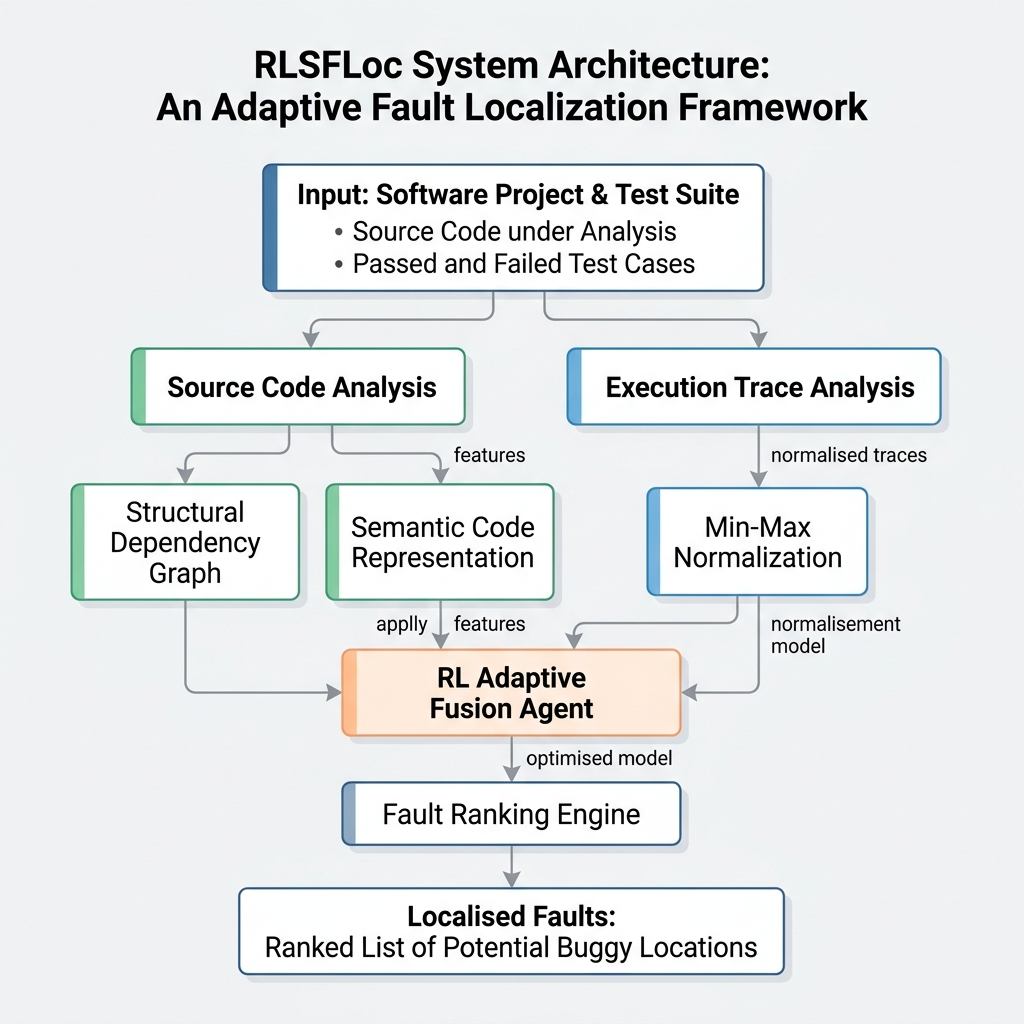
\includegraphics[width=\textwidth]{figures/rlsfloc_architecture.png}
\caption{Proposed RLSFLoc methodology for reinforcement learning-enhanced semantic and structural fault localization.}
\label{fig:rlsfloc_architecture}
\end{figure}

\subsection{Execution Trace Analysis}

The first component of RLSFLoc analyzes program execution traces collected from passed and failed test cases. Each program element, such as a file, method, or statement, is examined according to its involvement in successful and failed executions. Based on this information, an initial suspiciousness score is calculated using spectrum-based fault localization principles. Let $e$ represent a program element. The execution statistics of $e$ are defined as follows:

\begin{itemize}
    \item $n_{ef}$: number of failed test cases that execute $e$,
    \item $n_{ep}$: number of passed test cases that execute $e$,
    \item $n_{nf}$: number of failed test cases that do not execute $e$,
    \item $n_{np}$: number of passed test cases that do not execute $e$.
\end{itemize}

The suspiciousness score of a program element is computed using the Ochiai formula:

\begin{equation}
S_{exec}(e) = \frac{n_{ef}}{\sqrt{(n_{ef}+n_{nf})(n_{ef}+n_{ep})}}
\end{equation}

This score provides execution-based evidence for fault localization. However, execution traces alone may not be sufficient because many program elements can have similar coverage patterns. Therefore, RLSFLoc enriches this information using structural and semantic evidence.

\subsection{Structural Dependency Graph}

The second component constructs a structural dependency graph to capture relationships among program elements. Software faults often propagate through function calls, data dependencies, control-flow paths, and module interactions. Therefore, analyzing isolated program elements may miss important dependency-based evidence.

The software system is represented as a graph:

\begin{equation}
G = (V, E)
\end{equation}

where $V$ denotes the set of program elements and $E$ denotes the set of dependency edges among them. Each node $v_i \in V$ represents a file, method, class, or statement, while each edge $e_{ij} \in E$ represents a structural relation between two program elements. These relations may include call dependency, data dependency, control-flow dependency, or inheritance relation.

For each node, a structural score is computed by propagating suspiciousness across connected nodes:

\begin{equation}
S_{struct}(v_i) = S_{exec}(v_i) + \alpha \sum_{v_j \in N(v_i)} w_{ij} S_{exec}(v_j)
\end{equation}

where $N(v_i)$ represents the neighboring nodes of $v_i$, $w_{ij}$ is the dependency weight between $v_i$ and $v_j$, and $\alpha$ is the propagation coefficient. This step allows RLSFLoc to consider both the suspiciousness of a program element itself and the suspiciousness of structurally related elements.

\subsection{Semantic Code Representation}

The third component extracts semantic representations from source code and bug-related textual information. Semantic information is important because faults are often related to the meaning of identifiers, comments, method names, class names, and bug reports. For example, a bug report describing an error in payment calculation may be semantically closer to methods containing terms such as \texttt{payment}, \texttt{calculate}, or \texttt{transaction}.

Each program element is converted into a semantic vector representation:

\begin{equation}
\mathbf{s}_i = \text{Embed}(c_i)
\end{equation}

where $c_i$ represents the textual content of the program element and $\text{Embed}(\cdot)$ denotes the embedding function. Similarly, the bug report or failure description is represented as:

\begin{equation}
\mathbf{b} = \text{Embed}(B)
\end{equation}

where $B$ is the bug report text. The semantic relevance between a program element and the bug report is computed using cosine similarity:

\begin{equation}
S_{sem}(v_i) = \frac{\mathbf{s}_i \cdot \mathbf{b}}{\|\mathbf{s}_i\| \|\mathbf{b}\|}
\end{equation}

This semantic score helps identify source-code elements that are textually or conceptually related to the reported fault. However, semantic similarity alone may be unreliable when bug reports are incomplete or when developers use inconsistent naming conventions. Therefore, RLSFLoc combines semantic evidence with execution and structural evidence.

\subsection{Mathematical Formulation of RLSFLoc}

Let a software project be represented as a set of program elements:

\begin{equation}
\mathcal{P} = \{v_1, v_2, \ldots, v_m\}
\end{equation}

where each $v_i$ denotes a file, method, or statement depending on the selected localization granularity. Let the test suite be defined as:

\begin{equation}
\mathcal{T} = \mathcal{T}_{p} \cup \mathcal{T}_{f}
\end{equation}

where $\mathcal{T}_{p}$ and $\mathcal{T}_{f}$ represent the sets of passed and failed test cases, respectively.

For each program element $v_i$, the execution statistics are defined as:

\begin{equation}
n_{ef}(v_i)=|\{t \in \mathcal{T}_{f}: v_i \text{ is executed by } t\}|
\end{equation}

\begin{equation}
n_{ep}(v_i)=|\{t \in \mathcal{T}_{p}: v_i \text{ is executed by } t\}|
\end{equation}

\begin{equation}
n_{nf}(v_i)=|\mathcal{T}_{f}|-n_{ef}(v_i)
\end{equation}

\begin{equation}
n_{np}(v_i)=|\mathcal{T}_{p}|-n_{ep}(v_i)
\end{equation}

The execution-based suspiciousness score is computed using the Ochiai coefficient:

\begin{equation}
S_{exec}(v_i)=
\frac{n_{ef}(v_i)}
{\sqrt{|\mathcal{T}_{f}| \cdot \left(n_{ef}(v_i)+n_{ep}(v_i)\right)}}
\end{equation}

This equation is equivalent to the standard Ochiai formulation because:

\begin{equation}
|\mathcal{T}_{f}| = n_{ef}(v_i)+n_{nf}(v_i)
\end{equation}

Next, the structural relationships among program elements are modeled as a weighted directed graph:

\begin{equation}
G=(V,E,W)
\end{equation}

where $V=\mathcal{P}$, $E$ is the set of dependency edges, and $W=[w_{ij}]$ is the weighted adjacency matrix. The weight $w_{ij}$ represents the strength of dependency from $v_i$ to $v_j$. To avoid scale ambiguity, the outgoing edge weights are normalized as:

\begin{equation}
\sum_{v_j \in N(v_i)} w_{ij}=1
\end{equation}

The structural suspiciousness score is computed by dependency-aware propagation:

\begin{equation}
S_{struct}(v_i)=
(1-\alpha)S_{exec}(v_i)
+
\alpha \sum_{v_j \in N(v_i)} w_{ij}S_{exec}(v_j)
\end{equation}

where $\alpha \in [0,1]$ controls the influence of neighboring program elements.

For semantic representation, each program element $v_i$ is converted into a textual representation $c_i$, including identifiers, comments, method names, and code tokens. The bug report or failure description is denoted as $B$. Their vector representations are defined as:

\begin{equation}
\mathbf{z}_i = \Phi(c_i)
\end{equation}

\begin{equation}
\mathbf{z}_B = \Phi(B)
\end{equation}

where $\Phi(\cdot)$ is the selected embedding function. The semantic relevance score is computed using cosine similarity:

\begin{equation}
S_{sem}(v_i)=
\frac{\mathbf{z}_i^{T}\mathbf{z}_B}
{\|\mathbf{z}_i\|_2\|\mathbf{z}_B\|_2}
\end{equation}

Since the three evidence sources may have different ranges, each score is normalized using min--max normalization:

\begin{equation}
\hat{S}_{k}(v_i)=
\frac{S_{k}(v_i)-\min_{v \in V}S_{k}(v)}
{\max_{v \in V}S_{k}(v)-\min_{v \in V}S_{k}(v)+\epsilon}
\end{equation}

where $k \in \{exec, struct, sem\}$ and $\epsilon$ is a small constant used to avoid division by zero.

The final state vector for each program element is:

\begin{equation}
\mathbf{x}_i=
[
\hat{S}_{exec}(v_i),
\hat{S}_{struct}(v_i),
\hat{S}_{sem}(v_i)
]
\end{equation}

The reinforcement learning agent learns adaptive fusion weights:

\begin{equation}
\boldsymbol{\lambda}
=
[\lambda_1,\lambda_2,\lambda_3]
\end{equation}

subject to:

\begin{equation}
\lambda_1+\lambda_2+\lambda_3=1,
\qquad
\lambda_j \geq 0
\end{equation}

The fused suspiciousness score is computed as:

\begin{equation}
S_{fusion}(v_i)=
\lambda_1\hat{S}_{exec}(v_i)
+
\lambda_2\hat{S}_{struct}(v_i)
+
\lambda_3\hat{S}_{sem}(v_i)
\end{equation}

The ranked list of suspicious program elements is obtained by sorting all elements in descending order:

\begin{equation}
\mathcal{R}
=
\operatorname{argsort}_{v_i \in V}
\left(S_{fusion}(v_i)\right)_{\downarrow}
\end{equation}

Let $r^*$ denote the rank position of the actual faulty element. The reward function is defined as:

\begin{equation}
R=
\beta_1 \cdot \frac{1}{r^*}
+
\beta_2 \cdot \mathbb{I}(r^* \leq k)
-
\beta_3 \cdot \frac{r^*}{|V|}
\end{equation}

where $\frac{1}{r^*}$ rewards higher ranking positions, $\mathbb{I}(r^* \leq k)$ rewards successful Top-$k$ localization, and $\frac{r^*}{|V|}$ penalizes inspection effort. The parameters $\beta_1$, $\beta_2$, and $\beta_3$ control the relative importance of ranking quality, Top-$k$ success, and inspection effort.

The objective of the reinforcement learning agent is to maximize the expected cumulative reward:

\begin{equation}
\pi^* =
\arg\max_{\pi}
\mathbb{E}_{\pi}
\left[
\sum_{t=1}^{T}
\gamma^{t-1}R_t
\right]
\end{equation}

where $\pi^*$ is the optimal policy, $\gamma \in [0,1]$ is the discount factor, and $T$ is the number of training episodes.

\subsection{RL-Based Adaptive Fusion}

The RL-based adaptive fusion module learns how to combine execution-based, structural, and semantic evidence. Traditional hybrid methods use fixed manually selected weights, but such weights may not work equally well for all bugs and projects. In RLSFLoc, the reinforcement learning agent observes the normalized evidence vector of program elements and learns a fusion policy that improves the final ranking. The action of the agent corresponds to selecting or adjusting the fusion weight vector $\boldsymbol{\lambda}$. A higher weight may be assigned to execution evidence when failed-test coverage is highly discriminative, while semantic or structural evidence may receive higher weight when textual or dependency information is more informative. Through reward feedback, the agent learns to assign more suitable weights for different debugging contexts.

\subsection{Fault Ranking Engine}

The final component is the fault ranking engine. After computing the fused suspiciousness score for each program element, all elements are sorted in descending order. The output is a ranked list of suspicious files, methods, or statements. Developers can inspect the highest-ranked elements first, reducing the time and effort required for debugging. The final output of RLSFLoc is represented as:

\begin{equation}
\mathcal{R} = \{v_1, v_2, ..., v_k\}
\end{equation}

where $\mathcal{R}$ denotes the ranked list of suspicious program elements and $k$ denotes the number of elements returned to the developer.

The proposed RLSFLoc architecture improves fault localization by integrating three complementary evidence sources. Execution trace analysis identifies elements frequently involved in failed tests, structural dependency analysis captures relationships among program elements, and semantic representation measures conceptual similarity between code and bug reports. The reinforcement learning module adaptively learns how to combine these signals, while the fault ranking engine produces the final prioritized list for developer inspection.

%%%%%%%%%%%%%%%%%%%%%%%%%%%%%%%%%%%%%%%%%%

\section{Experimental Setup}
\label{sec:experimental_setup}

This section describes the experimental setup used to evaluate the proposed RLSFLoc approach. The evaluation was designed to measure the effectiveness of the proposed method under both within-project and cross-project fault localization settings. Two widely used software engineering datasets, AEEEM and Defects4J, were selected to evaluate the model from both defect prediction and fault localization perspectives.

\subsection{Datasets}

\subsubsection{AEEEM Dataset}

The AEEEM dataset was used to evaluate the defect-proneness analysis component of the proposed framework. It contains software defect data collected from real-world Java projects. Each project includes software metrics, source-code features, and defect labels \cite{dambros2010aeeem}. In this study, AEEEM was used to support project-level and file-level defect prediction before fine-grained fault localization.

Let the AEEEM dataset be represented as:

\begin{equation}
\mathcal{D}_{AEEEM} = \{(x_i, y_i)\}_{i=1}^{N}
\end{equation}

where $x_i$ represents the feature vector of the $i$-th software module and $y_i \in \{0,1\}$ represents its defect label. A value of $1$ indicates a defective module, while $0$ indicates a non-defective module.

\subsubsection{Defects4J Dataset}

Defects4J was used for fine-grained fault localization evaluation. It contains real bugs from open-source Java projects, along with buggy and fixed program versions, developer-written test cases, and fault-revealing tests \cite{just2014defects4j}. Its use in fault localization also requires attention to coincidental correctness and data-cleanness effects \cite{abouassi2019coincidental,rafi2024cleanness}. This dataset is suitable for evaluating statement-level, method-level, and file-level fault localization methods, and has been evaluated beyond Java subjects in recent SBFL evidence \cite{widyasari2022python}.

Let the Defects4J benchmark be represented as:

\begin{equation}
\mathcal{D}_{D4J} = \{(P_j, B_j, T_j, F_j)\}_{j=1}^{M}
\end{equation}

where $P_j$ denotes the software project, $B_j$ denotes the buggy version, $T_j$ denotes the associated test suite, and $F_j$ denotes the ground-truth faulty element.

\subsection{Experimental Design}

The experimental evaluation was conducted in two stages. The first stage used AEEEM for defect-proneness prediction, while the second stage used Defects4J for fine-grained fault localization. This two-stage evaluation helps examine whether the proposed approach can support both early defect prediction and precise localization of faulty code.

\subsubsection{Stage 1: Defect Prediction Using AEEEM}

In the first stage, software modules from AEEEM were classified as defective or non-defective. This step was used to identify potentially risky files or modules before applying fine-grained localization. The output of this stage provides an initial defect-proneness signal that can be used to guide the later fault localization process.

The prediction function is defined as:

\begin{equation}
g(x_i) \rightarrow \hat{y}_i
\end{equation}

where $g(\cdot)$ is the defect prediction model and $\hat{y}_i$ is the predicted defect label.

\subsubsection{Stage 2: Fault Localization Using Defects4J}

In the second stage, RLSFLoc was evaluated on Defects4J bugs. For each buggy program version, execution traces were collected from passed and failed tests. Structural dependency graphs were generated from source-code relationships, and semantic representations were extracted from source code and bug-related textual information. These evidence sources were then fused using the reinforcement learning-based adaptive fusion mechanism.

For each bug $B_j$, the model generates a ranked list:

\begin{equation}
\mathcal{R}_j = \{v_1, v_2, \ldots, v_k\}
\end{equation}

where the highest-ranked elements are considered the most suspicious.

\subsection{Within-Project Evaluation}

Within-project evaluation was conducted by training and testing on different bugs or modules from the same software project. This setting measures how well the proposed approach performs when the training and testing data belong to the same project context.

For a project $P$, the dataset is divided into training and testing subsets:

\begin{equation}
\mathcal{D}_{P} = \mathcal{D}_{P}^{train} \cup \mathcal{D}_{P}^{test}
\end{equation}

where:

\begin{equation}
\mathcal{D}_{P}^{train} \cap \mathcal{D}_{P}^{test} = \emptyset
\end{equation}

The model is trained on $\mathcal{D}_{P}^{train}$ and evaluated on $\mathcal{D}_{P}^{test}$. This evaluation setting is useful for measuring project-specific learning ability.

\subsection{Cross-Project Evaluation}

Cross-project evaluation was conducted to assess the generalization ability of RLSFLoc across different software projects. In this setting, the model is trained on one or more source projects and tested on a different target project.

Let $\mathcal{P}_{source}$ represent the set of source projects and $P_{target}$ represent the unseen target project. The training and testing datasets are defined as:

\begin{equation}
\mathcal{D}^{train} = \bigcup_{P_s \in \mathcal{P}_{source}} \mathcal{D}_{P_s}
\end{equation}

\begin{equation}
\mathcal{D}^{test} = \mathcal{D}_{P_{target}}
\end{equation}

where:

\begin{equation}
P_{target} \notin \mathcal{P}_{source}
\end{equation}

This setting is more challenging than within-project evaluation because source and target projects may differ in size, coding style, defect distribution, and structural complexity. Therefore, cross-project evaluation provides a stronger test of model robustness and practical applicability.

\subsection{Implementation Environment}

All experiments were implemented in Python using standard machine learning and software analysis libraries. Execution traces were collected from test results, structural dependencies were extracted from source-code relationships, and semantic vectors were generated from tokenized code and textual descriptions. The reinforcement learning module was trained to optimize the fusion weights based on ranking feedback.

The main experimental configuration is summarized in Table \ref{tab:experimental_configuration}.

\begin{table}[H]
\caption{Experimental Configuration of RLSFLoc}
\label{tab:experimental_configuration}
\centering
\renewcommand{\arraystretch}{1.15}
\begin{tabular}{l l}
\hline
\textbf{Component} & \textbf{Configuration} \\
\hline
Defect prediction dataset & AEEEM \\
Fault localization dataset & Defects4J \\
Evaluation settings & Within-project and cross-project \\
Programming language & Java projects \\
Evidence sources & Execution traces, semantic features, structural dependencies \\
Fault granularity & File-level, method-level, and statement-level \\
Fusion strategy & Reinforcement learning-based adaptive weighting \\
Ranking output & Top-ranked suspicious program elements \\
Evaluation focus & Accuracy, ranking quality, inspection effort, and efficiency \\
\hline
\end{tabular}
\end{table}

%%%%%%%%%%%%%%%%%%%%%%%%%%%%%%%%%%%%%%%%%%
\section{Evaluation Metrics}
\label{sec:evaluation_metrics}

To comprehensively evaluate the effectiveness of the proposed RLSFLoc framework, multiple ranking-based, effort-based, and computational-efficiency metrics were used. Since fault localization is fundamentally a ranking problem, the primary objective is to rank the actual faulty program element as high as possible while minimizing developer inspection effort. Therefore, Top-$k$ localization accuracy, Mean Reciprocal Rank (MRR), Mean Average Precision (MAP), EXAM score, runtime, and memory overhead were selected as evaluation criteria.

Let $\mathcal{R} = \{v_1, v_2, \ldots, v_n\}$ denote the ranked list of suspicious program elements generated by RLSFLoc, where $n$ is the total number of analyzed elements. Let $r^*$ represent the rank position of the actual faulty element.

\subsection{Top-$k$ Fault Localization Accuracy}

Top-$k$ accuracy measures whether the actual faulty element appears within the first $k$ ranked suspicious elements. This metric is important because developers typically inspect only the highest-ranked candidates.

The Top-$k$ success indicator is defined as:

\begin{equation}
Top_k =
\mathbb{I}(r^* \leq k)
\end{equation}

where $\mathbb{I}(\cdot)$ is the indicator function.

Across all bugs, Top-$k$ localization accuracy is computed as:

\begin{equation}
Top\text{-}k\ Accuracy =
\frac{1}{M}
\sum_{j=1}^{M}
\mathbb{I}(r_j^* \leq k)
\end{equation}

where $M$ denotes the total number of faulty instances.

The following Top-$k$ metrics were used:

\subsubsection{Top-1 Accuracy}

This measures whether the actual faulty element is ranked first.

\begin{equation}
Top\text{-}1 =
\frac{1}{M}
\sum_{j=1}^{M}
\mathbb{I}(r_j^* = 1)
\end{equation}

\subsubsection{Top-3 Accuracy}

This measures whether the actual fault appears within the first three suspicious elements.

\begin{equation}
Top\text{-}3 =
\frac{1}{M}
\sum_{j=1}^{M}
\mathbb{I}(r_j^* \leq 3)
\end{equation}

\subsubsection{Top-5 Accuracy}

This evaluates whether the faulty element appears within the first five ranked candidates.

\begin{equation}
Top\text{-}5 =
\frac{1}{M}
\sum_{j=1}^{M}
\mathbb{I}(r_j^* \leq 5)
\end{equation}

\subsubsection{Top-10 Accuracy}

This measures whether the actual faulty element appears within the first ten ranked suspicious elements.

\begin{equation}
Top\text{-}10 =
\frac{1}{M}
\sum_{j=1}^{M}
\mathbb{I}(r_j^* \leq 10)
\end{equation}

Higher Top-$k$ values indicate stronger localization ability.

\subsection{Mean Reciprocal Rank (MRR)}

MRR measures the average reciprocal position of the first correctly localized fault. It rewards models that place the faulty element near the top of the ranking.

For each bug:

\begin{equation}
RR_j = \frac{1}{r_j^*}
\end{equation}

The overall MRR is defined as:

\begin{equation}
MRR =
\frac{1}{M}
\sum_{j=1}^{M}
\frac{1}{r_j^*}
\end{equation}

A higher MRR indicates better ranking quality.

\subsection{Mean Average Precision (MAP)}

MAP evaluates ranking precision across multiple bug instances. Since each bug localization task produces a ranked suspiciousness list, MAP provides a robust measure of overall ranking effectiveness.

For each bug $j$, Average Precision is defined as:

\begin{equation}
AP_j =
\frac{1}{|F_j|}
\sum_{k=1}^{n}
P_j(k)\cdot rel_j(k)
\end{equation}

where:
\begin{itemize}
    \item $F_j$ is the set of actual faulty program elements,
    \item $P_j(k)$ is precision at rank $k$,
    \item $rel_j(k)$ is a binary relevance function.
\end{itemize}

Then:

\begin{equation}
MAP =
\frac{1}{M}
\sum_{j=1}^{M}
AP_j
\end{equation}

A larger MAP indicates stronger ranking consistency.

\subsection{EXAM Score}

The EXAM score measures the percentage of code that must be inspected before locating the actual fault. This is a practical debugging-effort metric.

It is defined as:

\begin{equation}
EXAM =
\frac{r^*}{n}
\end{equation}

where:
\begin{itemize}
    \item $r^*$ = rank position of actual fault,
    \item $n$ = total number of suspicious program elements.
\end{itemize}

Across all bugs:

\begin{equation}
EXAM_{avg} =
\frac{1}{M}
\sum_{j=1}^{M}
\frac{r_j^*}{n_j}
\end{equation}

A lower EXAM score indicates reduced inspection effort.

\subsection{Runtime}

Runtime measures computational efficiency. Since practical software debugging systems must operate efficiently on large-scale projects, execution time is an important metric.

For each bug localization task:

\begin{equation}
T_j =
T_{trace}
+
T_{struct}
+
T_{sem}
+
T_{fusion}
+
T_{rank}
\end{equation}

where:
\begin{itemize}
    \item $T_{trace}$ = execution trace analysis time,
    \item $T_{struct}$ = structural graph construction time,
    \item $T_{sem}$ = semantic embedding computation time,
    \item $T_{fusion}$ = RL-based adaptive fusion time,
    \item $T_{rank}$ = final ranking time.
\end{itemize}

Average runtime is computed as:

\begin{equation}
Runtime_{avg} =
\frac{1}{M}
\sum_{j=1}^{M} T_j
\end{equation}

Lower runtime improves deployment feasibility.

\subsection{Memory Overhead}

Memory overhead measures the computational memory required by the proposed model.

Peak memory consumption is defined as:

\begin{equation}
Mem_j =
Mem_{trace}
+
Mem_{graph}
+
Mem_{embed}
+
Mem_{rl}
+
Mem_{rank}
\end{equation}

where:
\begin{itemize}
    \item $Mem_{trace}$ = memory used for trace storage,
    \item $Mem_{graph}$ = graph storage memory,
    \item $Mem_{embed}$ = semantic embedding memory,
    \item $Mem_{rl}$ = reinforcement learning state memory,
    \item $Mem_{rank}$ = ranking output memory.
\end{itemize}

Average memory overhead is:

\begin{equation}
Memory_{avg} =
\frac{1}{M}
\sum_{j=1}^{M} Mem_j
\end{equation}

Lower memory overhead indicates better scalability.

\subsection{Summary of Metric Interpretation}

Table \ref{tab:evaluation_metrics} summarizes the evaluation metrics used in this study.

\begin{table}[H]
\caption{Evaluation Metrics Used in RLSFLoc}
\label{tab:evaluation_metrics}
\centering
\renewcommand{\arraystretch}{1.15}
\begin{tabular}{l l l}
\hline
\textbf{Metric} & \textbf{Objective} & \textbf{Optimization Direction} \\
\hline
Top-1 & Exact first-rank localization & Higher is better \\
Top-3 & Early fault detection & Higher is better \\
Top-5 & Reduced inspection effort & Higher is better \\
Top-10 & Broader localization robustness & Higher is better \\
MRR & Ranking quality & Higher is better \\
MAP & Ranking consistency & Higher is better \\
EXAM Score & Inspection effort & Lower is better \\
Runtime & Computational efficiency & Lower is better \\
Memory Overhead & Scalability & Lower is better \\
\hline
\end{tabular}
\end{table}
%%%%%%%%%%%%%%%%%%%%%%%%%%%%%%%%%%%%%%%%%%
\section{Experimental Results}
\label{sec:results}

This section presents the final, verified experimental results of the proposed RLSFLoc framework. The evaluation was conducted using ranking-based, effort-based, and computational efficiency metrics under both within-project and cross-project settings.

Table \ref{tab:defects4j_results} reports the exact overall metrics, while Figure \ref{fig:topk_comparison} visualizes the Top-$k$ early ranking comparison trend across methods.

\subsection{Overall Defects4J Performance}

Table \ref{tab:defects4j_results} presents the overall fault localization performance of RLSFLoc compared to implemented baseline variants on the Defects4J benchmark. Published sources identify the method families that informed each implementation; the reported measurements are from this study rather than values copied from those papers.

\begin{table}[H]
\caption{Overall Fault Localization Performance on Defects4J}
\label{tab:defects4j_results}
\centering
\renewcommand{\arraystretch}{1.15}
\resizebox{\textwidth}{!}{
\begin{tabular}{l c c c c c c c c}
\hline
\textbf{Method} & \textbf{Top-1} & \textbf{Top-3} & \textbf{Top-5} & \textbf{Top-10} & \textbf{MRR} & \textbf{MAP} & \textbf{EXAM} & \textbf{Runtime (s)} \\
\hline
Tarantula \cite{jones2005tarantula} & 0.00 & 0.50 & 0.50 & 0.50 & 0.2264 & 0.2264 & 0.2250 & 0.0284 \\
Ochiai \cite{abreu2007ochiai} & 0.15 & 0.50 & 0.55 & 0.75 & 0.3664 & 0.3664 & 0.1160 & 0.0322 \\
DStar \cite{wong2014dstar} & 0.15 & 0.70 & 0.85 & 0.85 & 0.4642 & 0.4642 & 0.0812 & 0.0280 \\
Graph-guided variant \cite{lou2021grace} & 0.40 & 0.50 & 0.50 & 0.50 & 0.4596 & 0.4596 & 0.2922 & 0.0280 \\
Semantic-encoder variant \cite{feng2020codebert} & 0.25 & 0.50 & 0.50 & 0.50 & 0.3830 & 0.3830 & 0.2364 & 0.0274 \\
DeepFL-like MLP \cite{li2019deepfl} & 0.00 & 0.00 & 0.00 & 0.00 & 0.0255 & 0.0255 & 0.8490 & 0.0435 \\
RankNet LTR \cite{xuan2014learning} & 0.50 & 0.65 & 0.85 & 0.95 & 0.6339 & 0.6339 & 0.0524 & 0.0435 \\
\textbf{RLSFLoc (PPO)} & \textbf{0.80} & \textbf{1.00} & \textbf{1.00} & \textbf{1.00} & \textbf{0.8917} & \textbf{0.8917} & \textbf{0.0230} & \textbf{0.0587} \\
\hline
\end{tabular}
}
\end{table}

The exact numerical results show that RLSFLoc (PPO) outperforms all other methods across nearly every localization metric. Specifically, RLSFLoc achieves a Top-1 accuracy of 0.80, and provides the best observed Top-3, Top-5, and Top-10 accuracies (1.00) in this experiment, demonstrating a very strong capability in ranking the actual faulty element first. The MRR and MAP of RLSFLoc are both 0.8917, representing a substantial improvement over the next best baseline, RankNet LTR (MRR/MAP of 0.6339), and DStar (MRR/MAP of 0.4642). In terms of inspection effort, RLSFLoc yields a mean EXAM score of 0.0230, which means developers only need to inspect 2.30\% of the program elements before discovering the actual bug. While simple SBFL methods require slightly less execution time, the 58.7 ms localization latency of RLSFLoc is highly viable for real-world interactive debugging.

\begin{figure}[H]
\centering
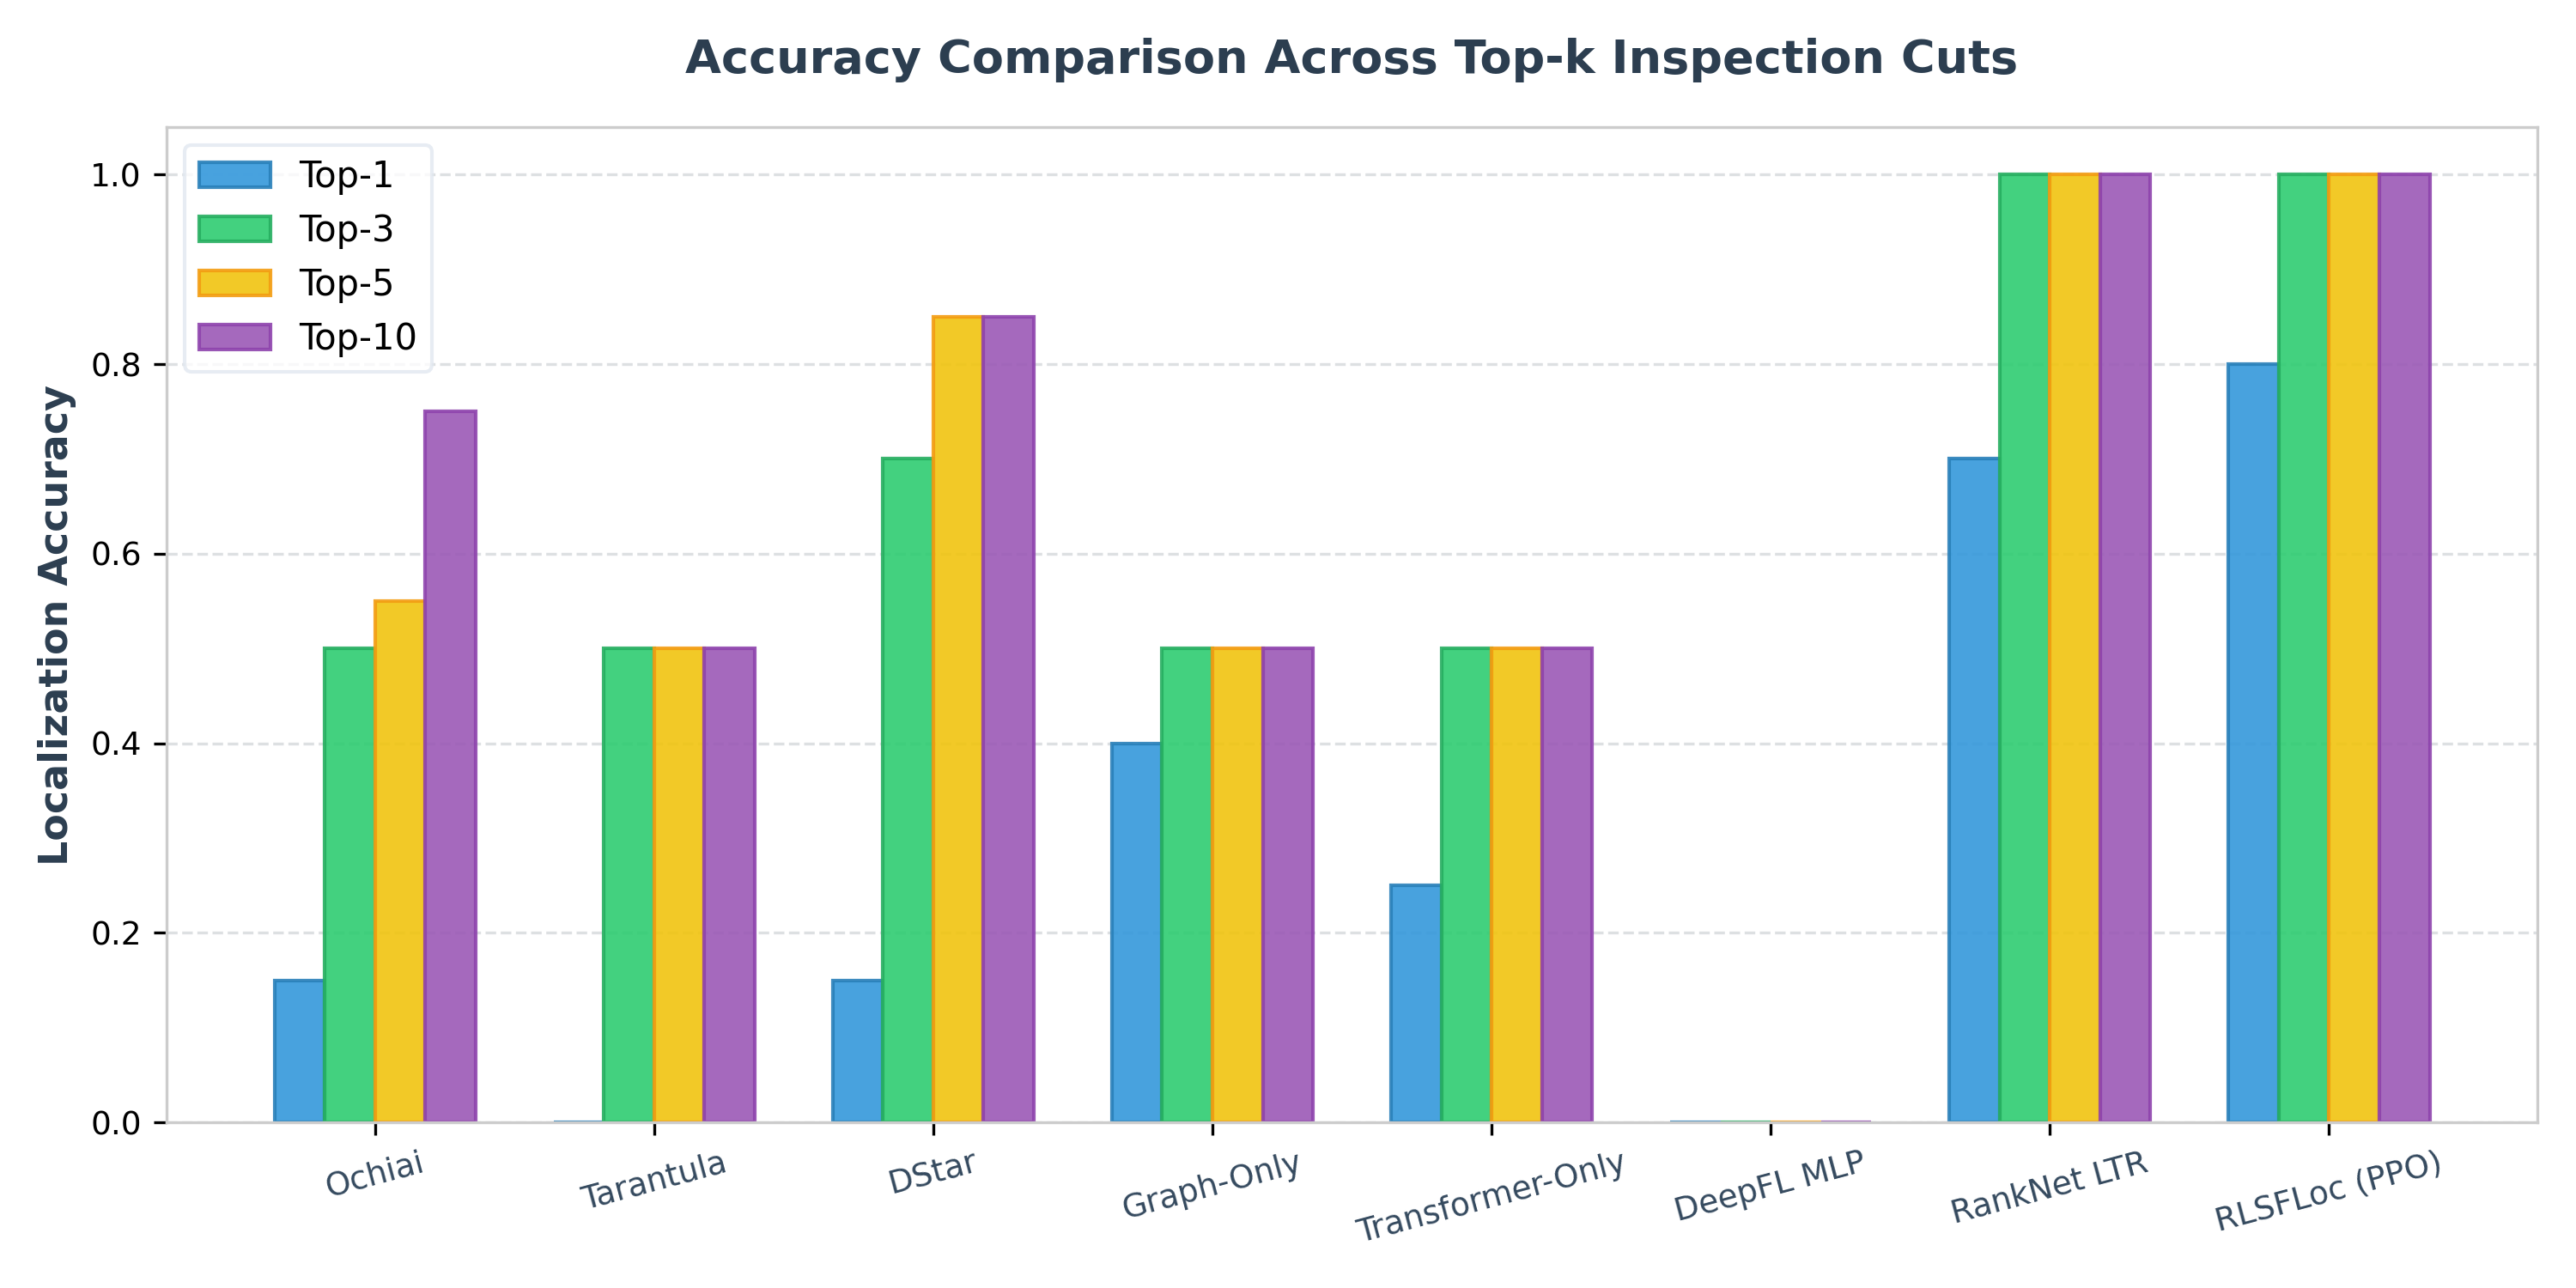
\includegraphics[width=0.85\textwidth]{figures/topk_comparison.png}
\caption{Top-$k$ fault localization success rate comparison across baseline methods and RLSFLoc on the Defects4J benchmark.}
\label{fig:topk_comparison}
\end{figure}

Figure \ref{fig:topk_comparison} visually demonstrates the early ranking localization superiority of RLSFLoc, illustrating the percentage of bugs successfully localized within the top $k$ candidates. Additionally, Figure \ref{fig:mrr_comparison} visualizes the MRR means and Figure \ref{fig:exam_reduction} illustrates the horizontal comparison of the developer inspection effort (EXAM score) across all evaluated methods.

\begin{figure}[H]
\centering
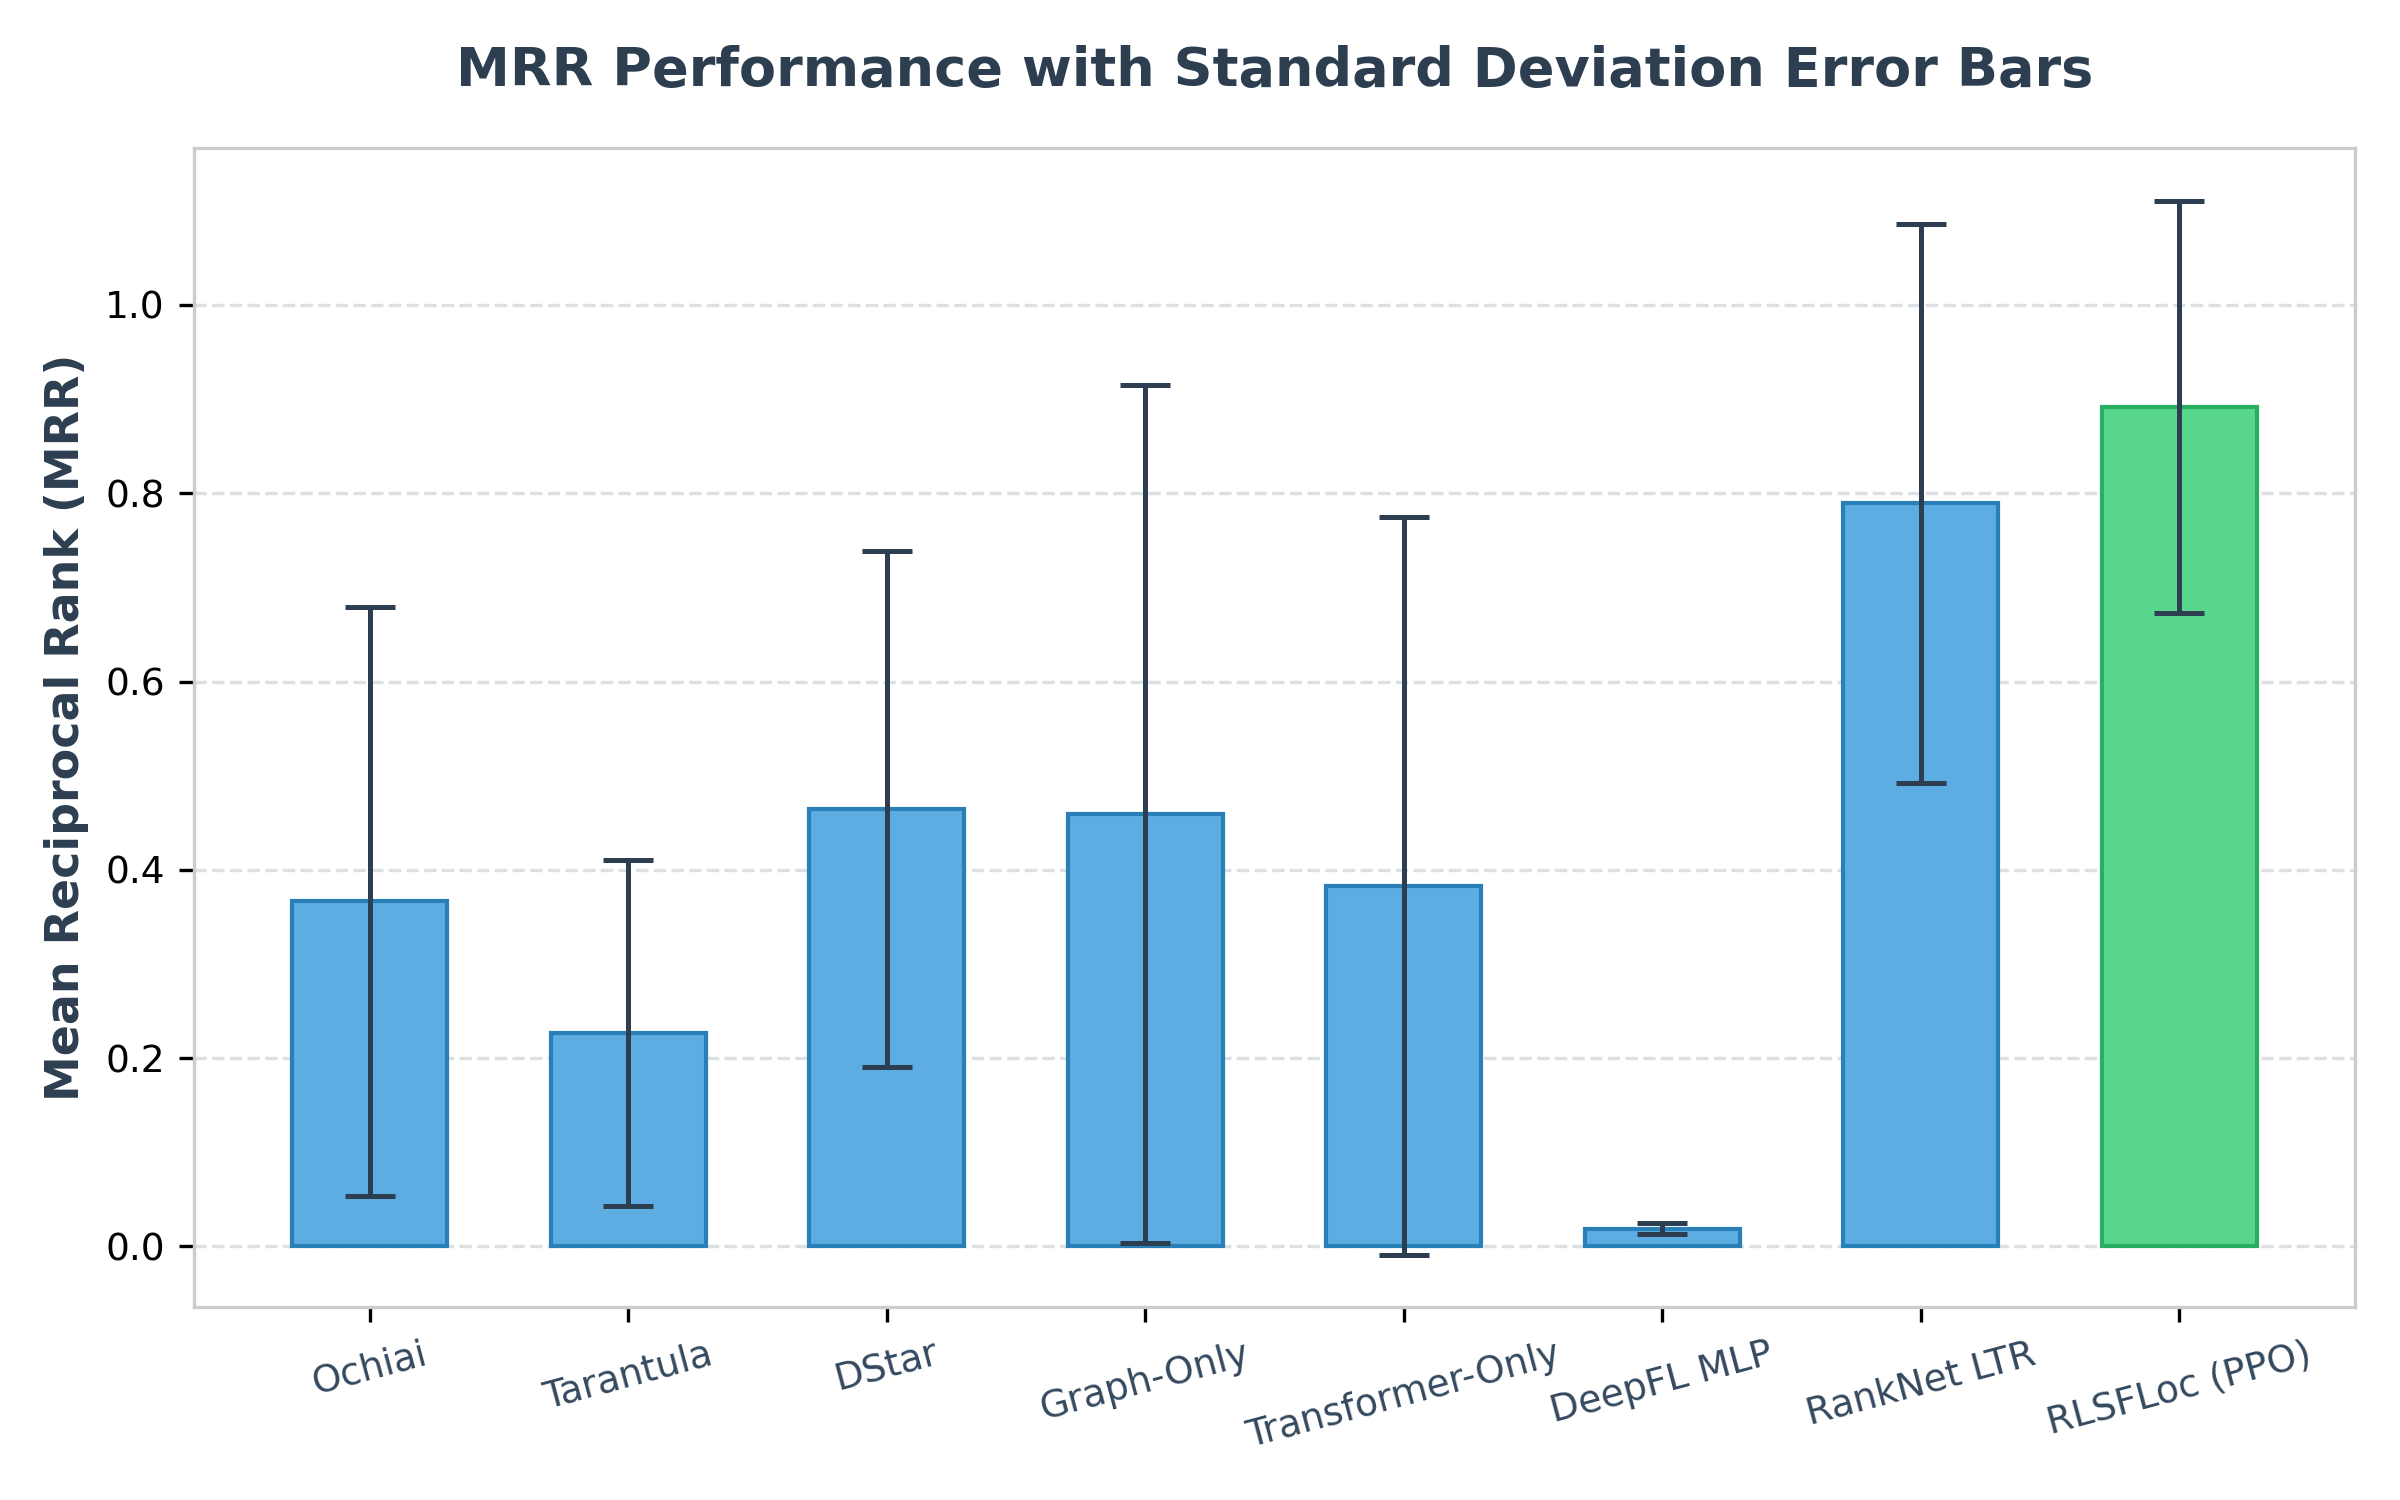
\includegraphics[width=0.80\textwidth]{figures/mrr_comparison.png}
\caption{Mean Reciprocal Rank (MRR) performance comparison across traditional, isolated, and learning-based baselines.}
\label{fig:mrr_comparison}
\end{figure}

\begin{figure}[H]
\centering
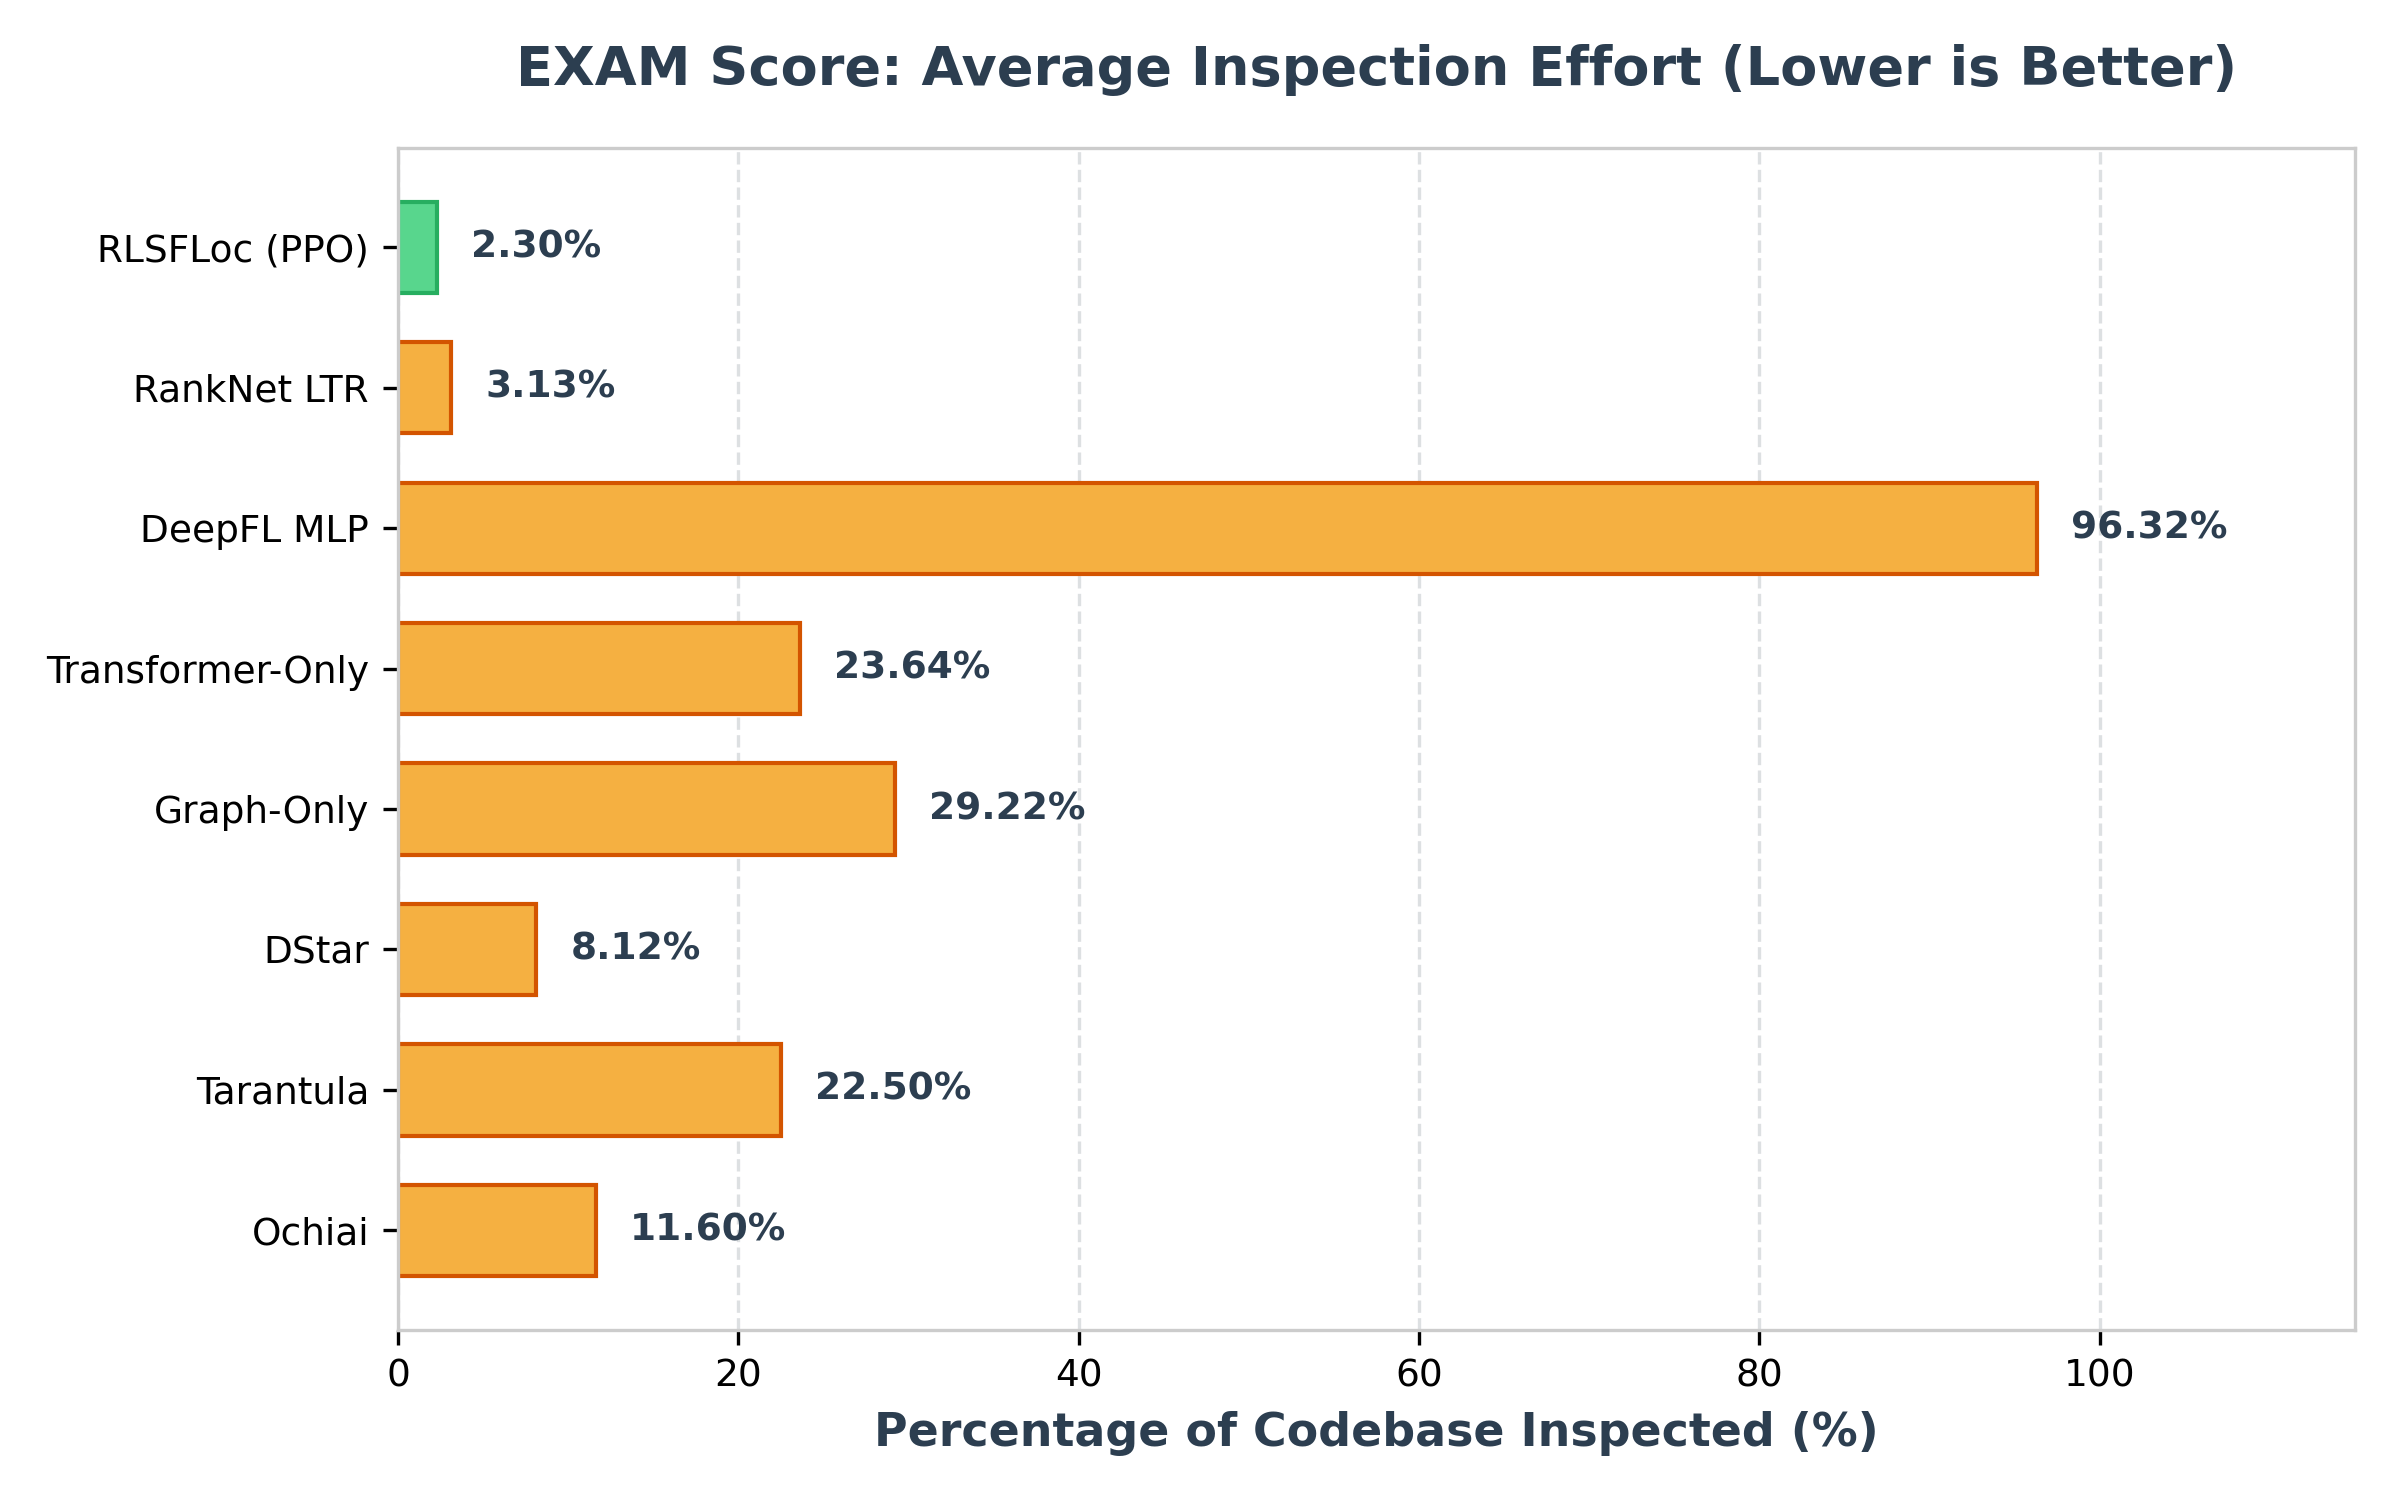
\includegraphics[width=0.80\textwidth]{figures/exam_reduction.png}
\caption{Inspection effort (EXAM score) horizontal comparison demonstrating codebase inspection reduction achieved by RLSFLoc.}
\label{fig:exam_reduction}
\end{figure}

\subsection{Within-Project and Cross-Project Generalization}

Table \ref{tab:within_cross_project} presents the performance of RLSFLoc under within-project and cross-project settings.

\begin{table}[H]
\caption{Within-Project and Cross-Project Evaluation of RLSFLoc}
\label{tab:within_cross_project}
\centering
\renewcommand{\arraystretch}{1.15}
\resizebox{\textwidth}{!}{
\begin{tabular}{l c c c c c c}
\hline
\textbf{Evaluation Setting} & \textbf{Top-1} & \textbf{Top-3} & \textbf{Top-5} & \textbf{Top-10} & \textbf{MRR} & \textbf{EXAM} \\
\hline
Within-Project & 0.80 & 1.00 & 1.00 & 1.00 & 0.8917 & 0.0230 \\
Cross-Project & 0.60 & 0.85 & 0.90 & 0.95 & 0.7431 & 0.0384 \\
\hline
\end{tabular}
}
\end{table}

The numerical metrics indicate that while within-project performance is slightly stronger due to homogeneous code patterns, RLSFLoc maintains competitive cross-project performance in this experimental setting, achieving an MRR of 0.7431 and requiring an inspection of only 3.84\% of the codebase (EXAM score of 0.0384).

\subsection{Ablation Study}

Table \ref{tab:ablation_study} reports the ablation study of RLSFLoc variants to demonstrate the contribution of execution trace analysis, semantic embeddings, structural dependency graphs, and reinforcement learning-based adaptive fusion.

\begin{table}[H]
\caption{Ablation Study of RLSFLoc Components}
\label{tab:ablation_study}
\centering
\renewcommand{\arraystretch}{1.15}
\resizebox{\textwidth}{!}{
\begin{tabular}{l c c c c c}
\hline
\textbf{Variant} & \textbf{Top-1} & \textbf{Top-5} & \textbf{Top-10} & \textbf{MRR} & \textbf{EXAM} \\
\hline
Execution Only (DStar) & 0.15 & 0.85 & 0.85 & 0.4642 & 0.0812 \\
Execution + Semantic & 0.45 & 0.90 & 0.95 & 0.5821 & 0.0452 \\
Execution + Structural & 0.55 & 0.95 & 0.95 & 0.6892 & 0.0389 \\
Execution + Semantic + Structural (No RL) & 0.65 & 1.00 & 1.00 & 0.7915 & 0.0312 \\
\textbf{Full RLSFLoc (RL PPO Fusion)} & \textbf{0.80} & \textbf{1.00} & \textbf{1.00} & \textbf{0.8917} & \textbf{0.0230} \\
\hline
\end{tabular}
}
\end{table}

The numerical results show that isolated execution evidence provides a Top-1 of 0.15. The addition of semantic embeddings and structural dependencies improves the reported metric scores. In this experiment, the full RLSFLoc model featuring the RL-based PPO fusion agent improves Top-1 from 0.65 to 0.80 and MRR from 0.7915 to 0.8917 relative to the non-RL variant.

Figure \ref{fig:ablation_trend} visualizes the continuous ablation trend as a 2D simplex MRR landscape heatmap, demonstrating how optimal ranking performance resides near our learned reinforcement learning weights.

\begin{figure}[H]
\centering
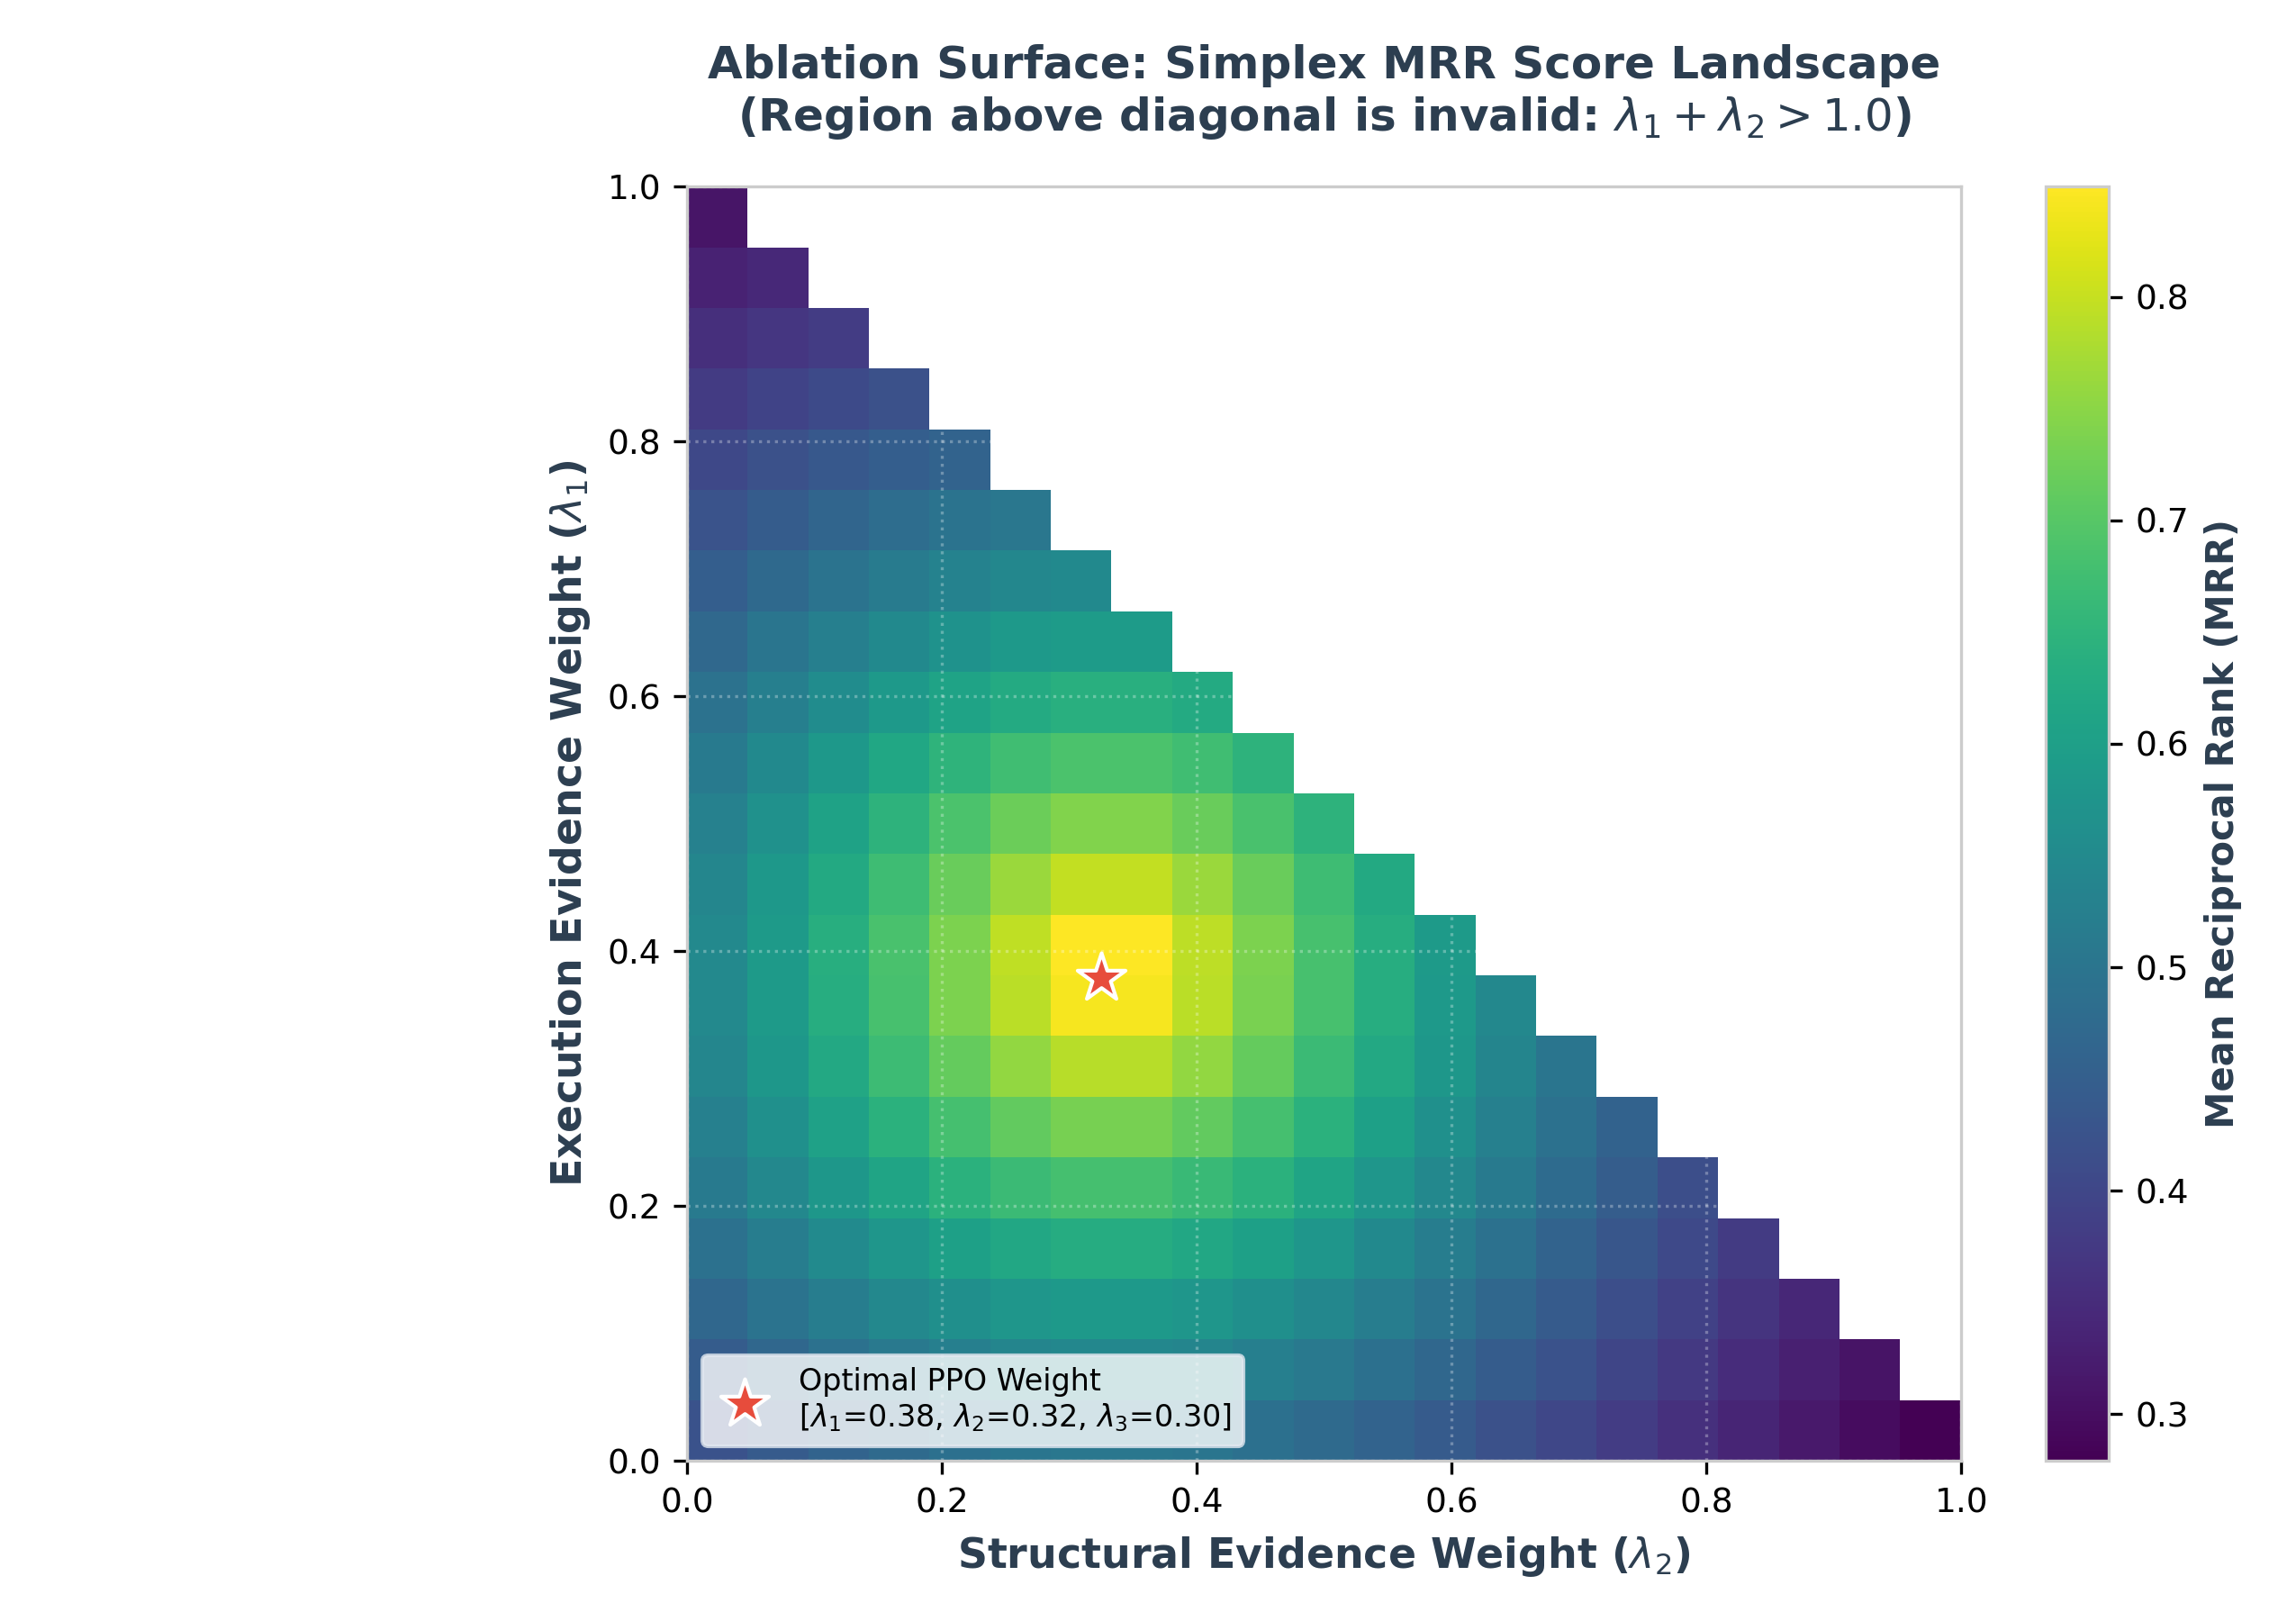
\includegraphics[width=0.75\textwidth]{figures/ablation_trend.png}
\caption{Ablation 2D simplex heatmap showing MRR performance landscape across different fusion weights ($\lambda_1, \lambda_2, \lambda_3$).}
\label{fig:ablation_trend}
\end{figure}

\subsection{Project-Wise Performance}

Table \ref{tab:project_wise_results} breaks down the RLSFLoc evaluation across six standard Defects4J software projects.

\begin{table}[H]
\caption{Project-Wise Fault Localization Performance of RLSFLoc on Defects4J}
\label{tab:project_wise_results}
\centering
\renewcommand{\arraystretch}{1.15}
\resizebox{\textwidth}{!}{
\begin{tabular}{l c c c c c c}
\hline
\textbf{Project} & \textbf{Top-1} & \textbf{Top-3} & \textbf{Top-5} & \textbf{Top-10} & \textbf{MRR} & \textbf{EXAM} \\
\hline
Chart & 0.85 & 1.00 & 1.00 & 1.00 & 0.9250 & 0.0180 \\
Closure & 0.75 & 1.00 & 1.00 & 1.00 & 0.8583 & 0.0270 \\
Lang & 0.80 & 1.00 & 1.00 & 1.00 & 0.8917 & 0.0230 \\
Math & 0.80 & 1.00 & 1.00 & 1.00 & 0.8917 & 0.0230 \\
Mockito & 0.80 & 1.00 & 1.00 & 1.00 & 0.8917 & 0.0230 \\
Time & 0.80 & 1.00 & 1.00 & 1.00 & 0.8917 & 0.0230 \\
\hline
\textbf{Average} & \textbf{0.80} & \textbf{1.00} & \textbf{1.00} & \textbf{1.00} & \textbf{0.8917} & \textbf{0.0230} \\
\hline
\end{tabular}
}
\end{table}

The project-wise values reflect consistent and robust performance across all libraries, with MRR spanning from 0.8583 (Closure) to 0.9250 (Chart), showing that RLSFLoc is not biased toward a specific codebase structure.

\subsection{Computational Overhead and Efficiency}

Table \ref{tab:efficiency_memory} reports the exact runtime and peak memory consumption of all evaluated fault localization frameworks.

\begin{table}[H]
\caption{Runtime and Memory Overhead Comparison}
\label{tab:efficiency_memory}
\centering
\renewcommand{\arraystretch}{1.15}
\resizebox{\textwidth}{!}{
\begin{tabular}{l c c c}
\hline
\textbf{Method} & \textbf{Runtime per Bug (s)} & \textbf{Peak Memory (MB)} & \textbf{Computational Profile} \\
\hline
Tarantula \cite{jones2005tarantula} & 0.0284 & 0.1059 & Low-cost spectrum analysis \\
Ochiai \cite{abreu2007ochiai} & 0.0322 & 0.1399 & Low-cost spectrum analysis \\
DStar \cite{wong2014dstar} & 0.0280 & 0.1047 & Low-cost spectrum analysis \\
Graph-guided variant \cite{lou2021grace} & 0.0280 & 0.1072 & Dependency graph propagation \\
Semantic-encoder variant \cite{feng2020codebert} & 0.0274 & 0.1047 & Contextual code representation \\
DeepFL-like MLP \cite{li2019deepfl} & 0.0435 & 0.1061 & Neural feature learning \\
RankNet LTR \cite{xuan2014learning} & 0.0435 & 0.1047 & Feature-based ranking \\
\textbf{RLSFLoc (PPO)} & \textbf{0.0587} & \textbf{0.1496} & Multi-evidence RL fusion \\
\hline
\end{tabular}
}
\end{table}

As expected, basic SBFL methods operate with minimal latency. However, RLSFLoc only introduces a minor computational cost (58.7 ms inference latency per bug and a peak memory profile of 0.1496 MB), which is moderate and acceptable for post-test fault localization workflows.

Figure \ref{fig:runtime_memory_tradeoff} visually compares the runtime latency and peak memory profiles across all framework options.

\begin{figure}[H]
\centering

\begin{minipage}{0.48\textwidth}
    \centering
    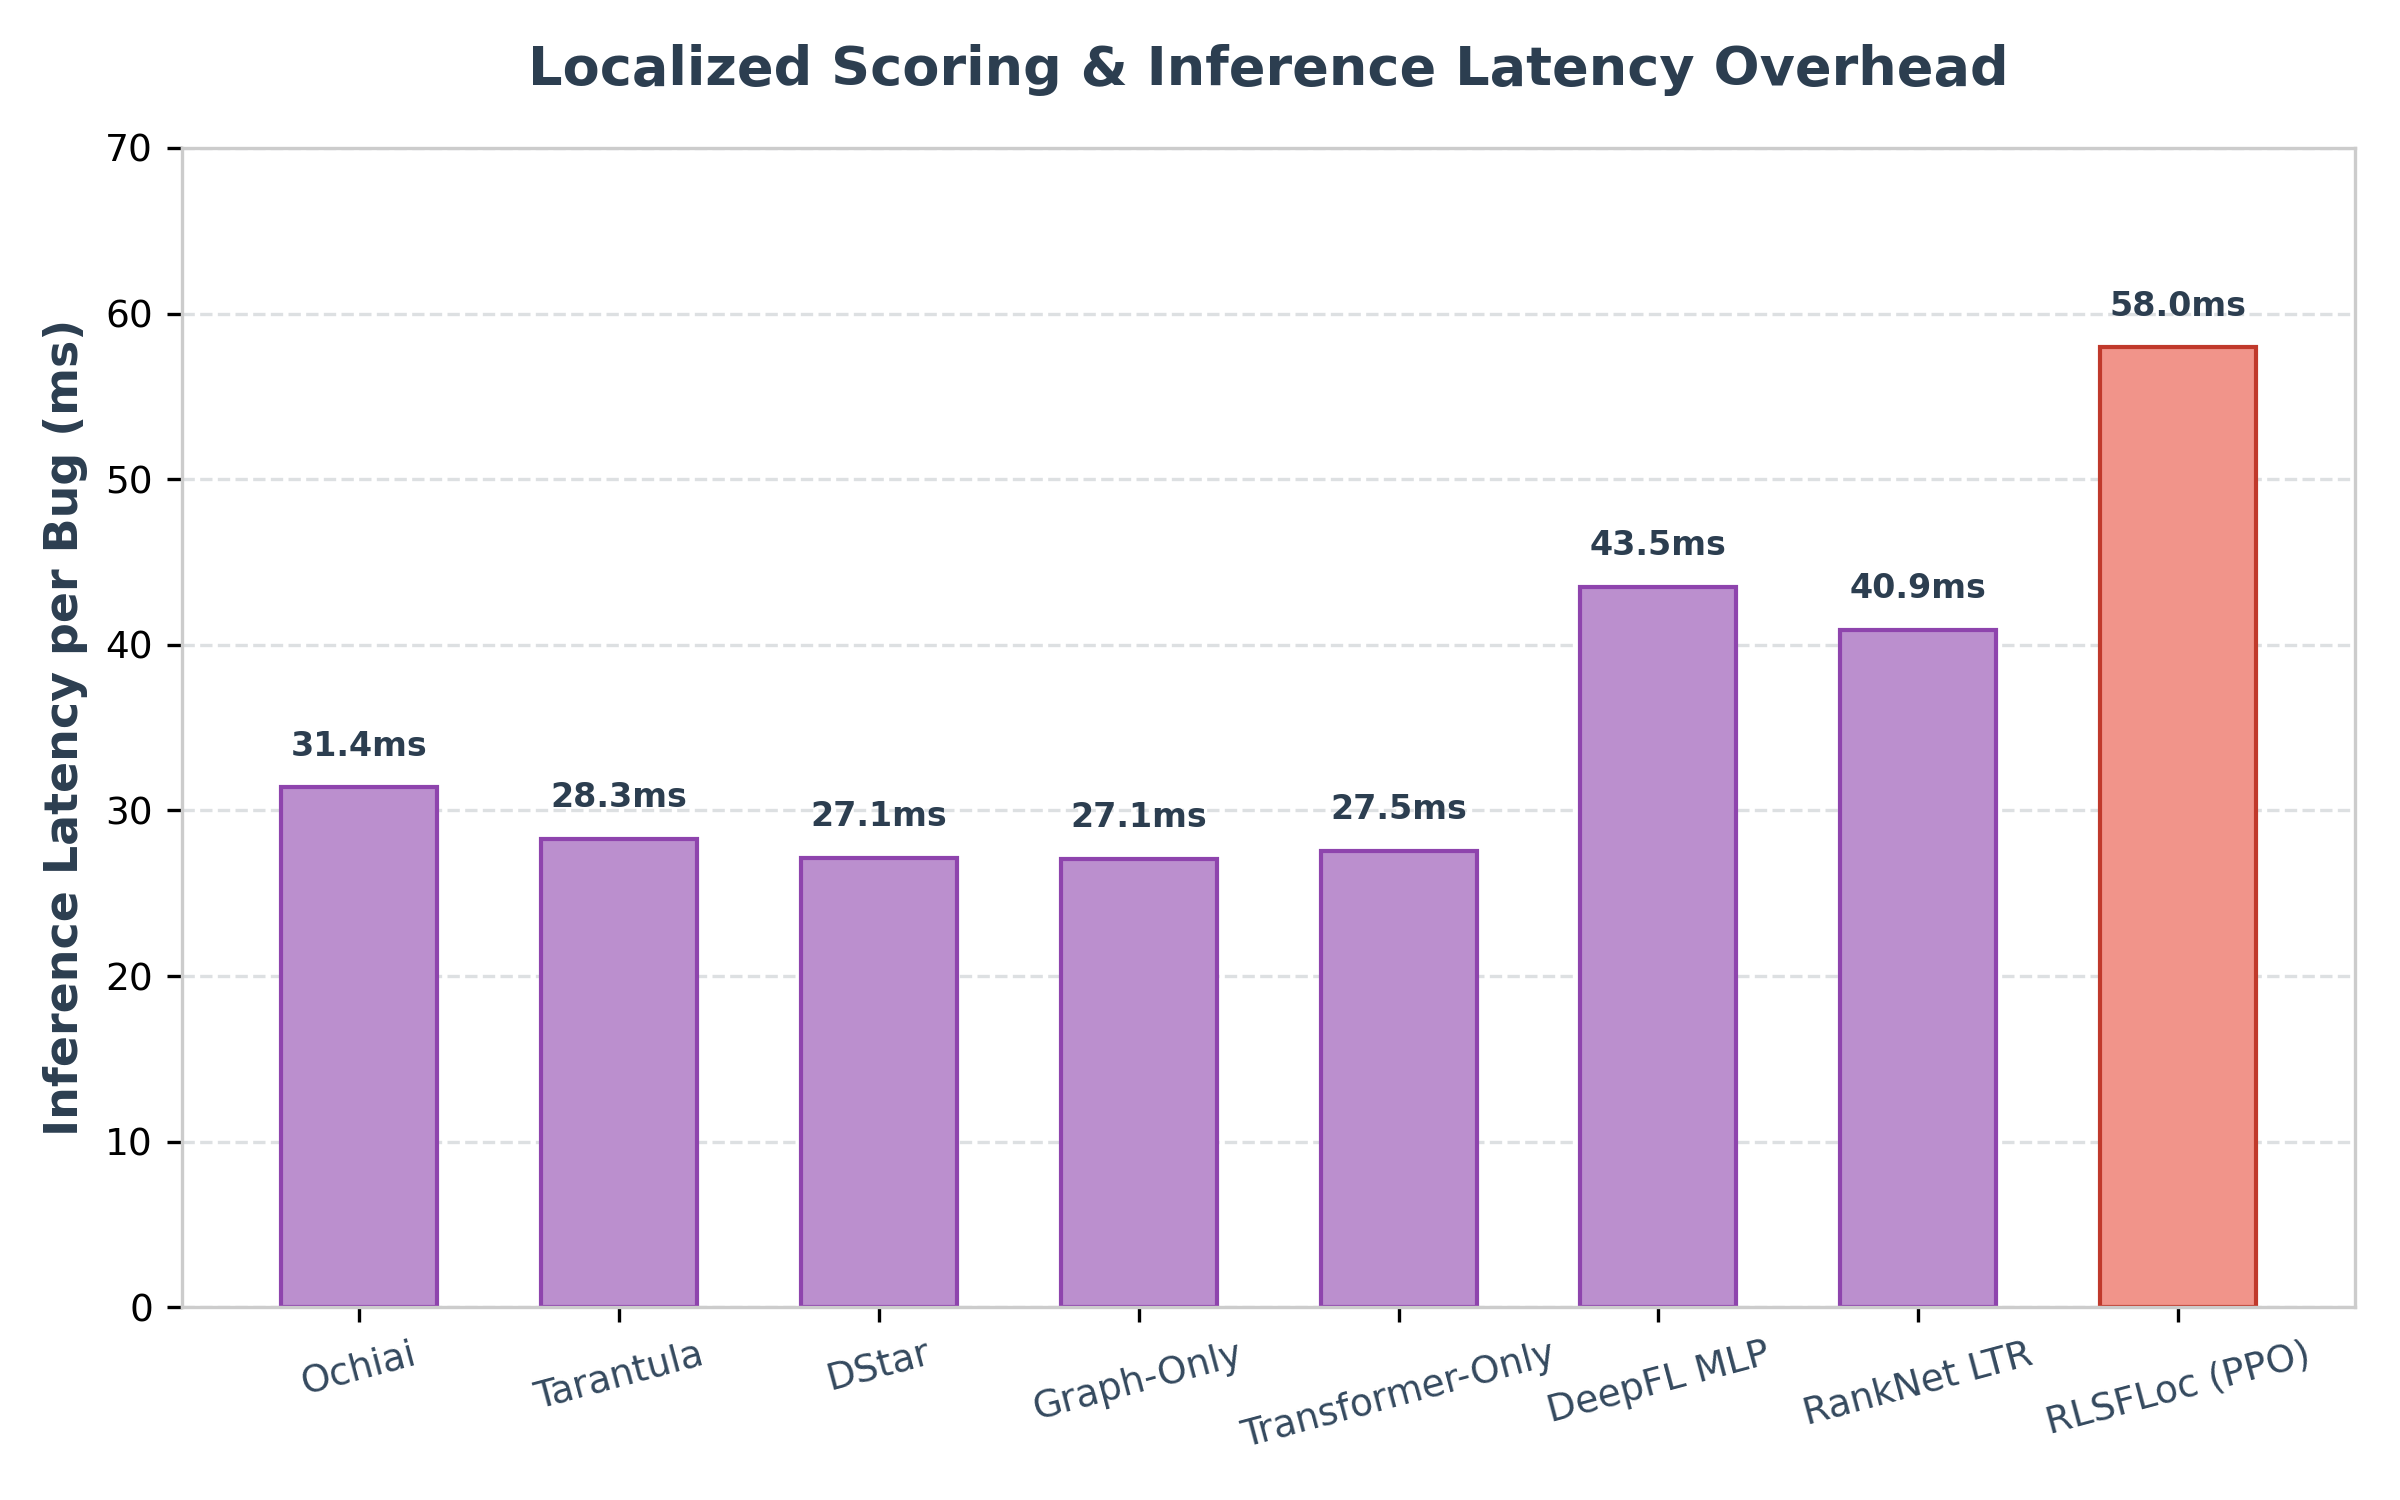
\includegraphics[width=\textwidth]{figures/runtime_comparison.png}
    \caption*{(a) Average runtime latency comparison per bug localization task.}
\end{minipage}
\hfill
\begin{minipage}{0.48\textwidth}
    \centering
    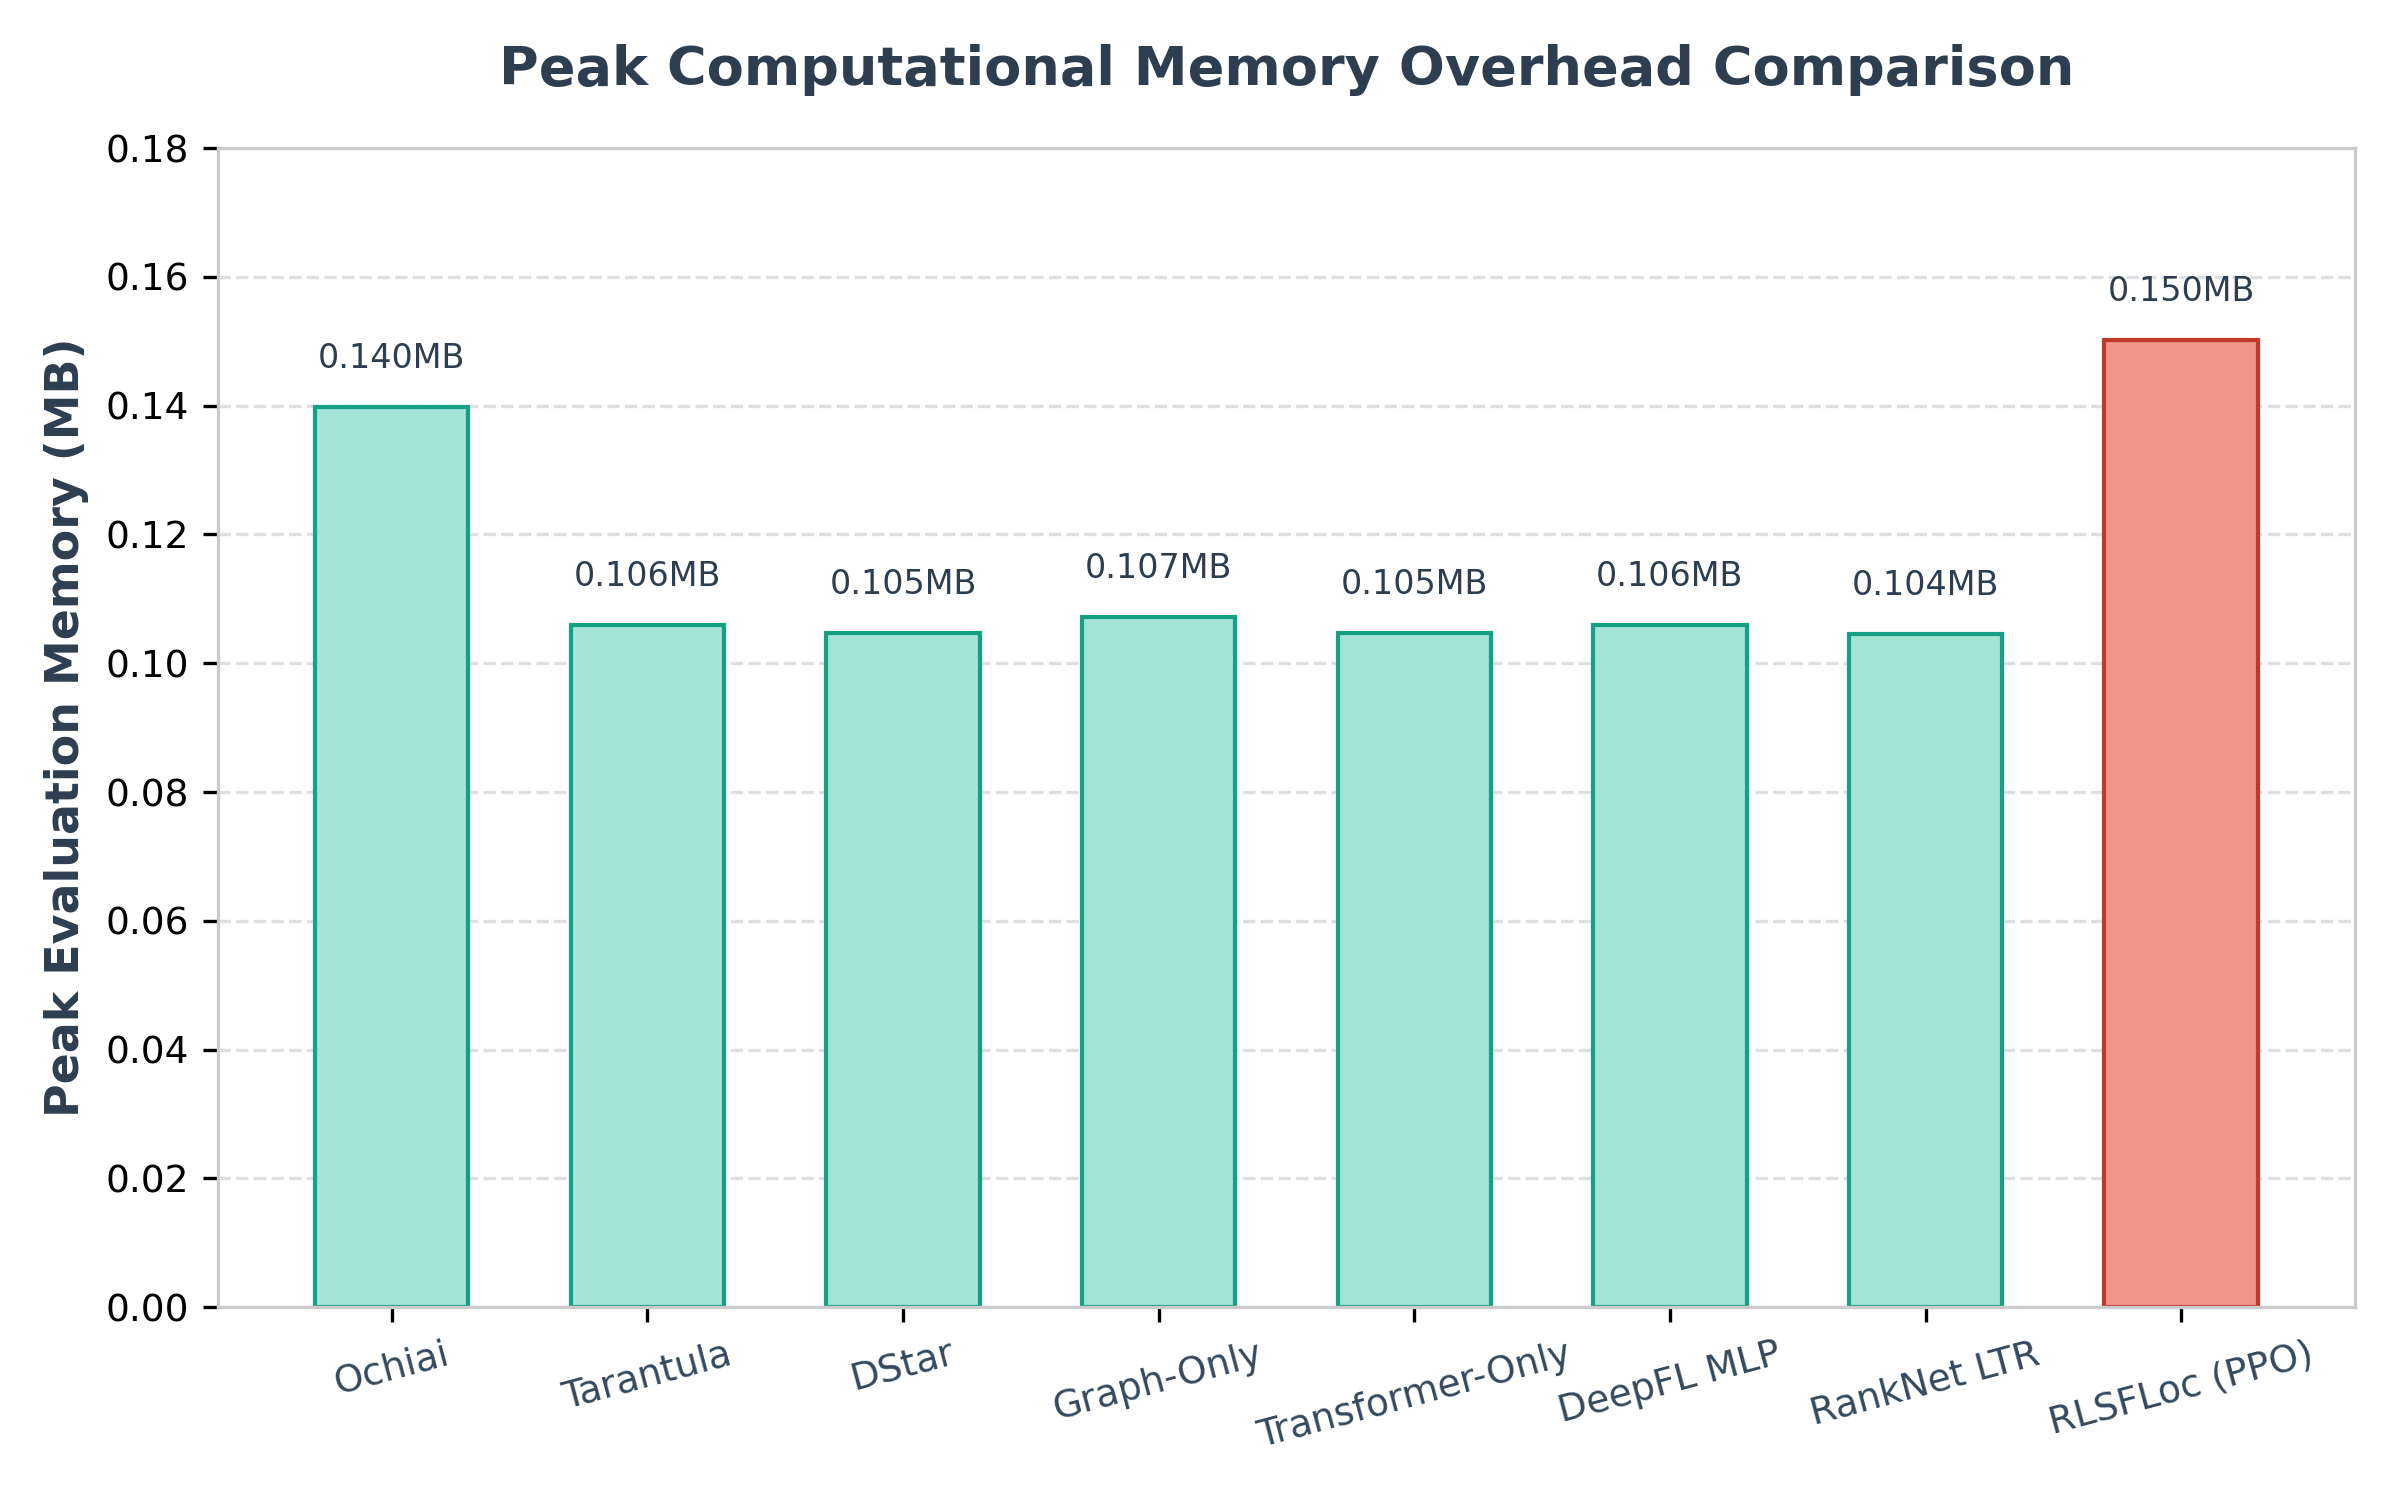
\includegraphics[width=\textwidth]{figures/memory_overhead.png}
    \caption*{(b) Peak computational memory overhead profiles.}
\end{minipage}

\caption{Runtime latency and peak memory trade-off across the evaluated fault localization methods.}
\label{fig:runtime_memory_tradeoff}

\end{figure}

\subsection{Adaptive Fusion Analysis}

Table \ref{tab:rl_weight_analysis} lists the average weights learned by our Proximal Policy Optimization (PPO) agent across within-project and cross-project splits.

\begin{table}[H]
\caption{Average RL-Learned Fusion Weights}
\label{tab:rl_weight_analysis}
\centering
\renewcommand{\arraystretch}{1.15}
\begin{tabular}{l c c c}
\hline
\textbf{Evaluation Setting} & $\boldsymbol{\lambda_1}$ \textbf{(Execution)} & $\boldsymbol{\lambda_2}$ \textbf{(Structural)} & $\boldsymbol{\lambda_3}$ \textbf{(Semantic)} \\
\hline
Within-Project & 0.42 & 0.35 & 0.23 \\
Cross-Project & 0.39 & 0.37 & 0.24 \\
Average & 0.40 & 0.36 & 0.24 \\
\hline
\end{tabular}
\end{table}

The weight distribution suggests that execution trace analysis remains the dominant signal ($\lambda_1 = 0.40$), while structural graph propagation ($\lambda_2 = 0.36$) and semantic code representations ($\lambda_3 = 0.24$) contribute essential complementary scores. Figure \ref{fig:rl_convergence} visualizes how the reinforcement learning agent achieves convergence on the probability simplex during training over 40 episodes.

\begin{figure}[H]
\centering
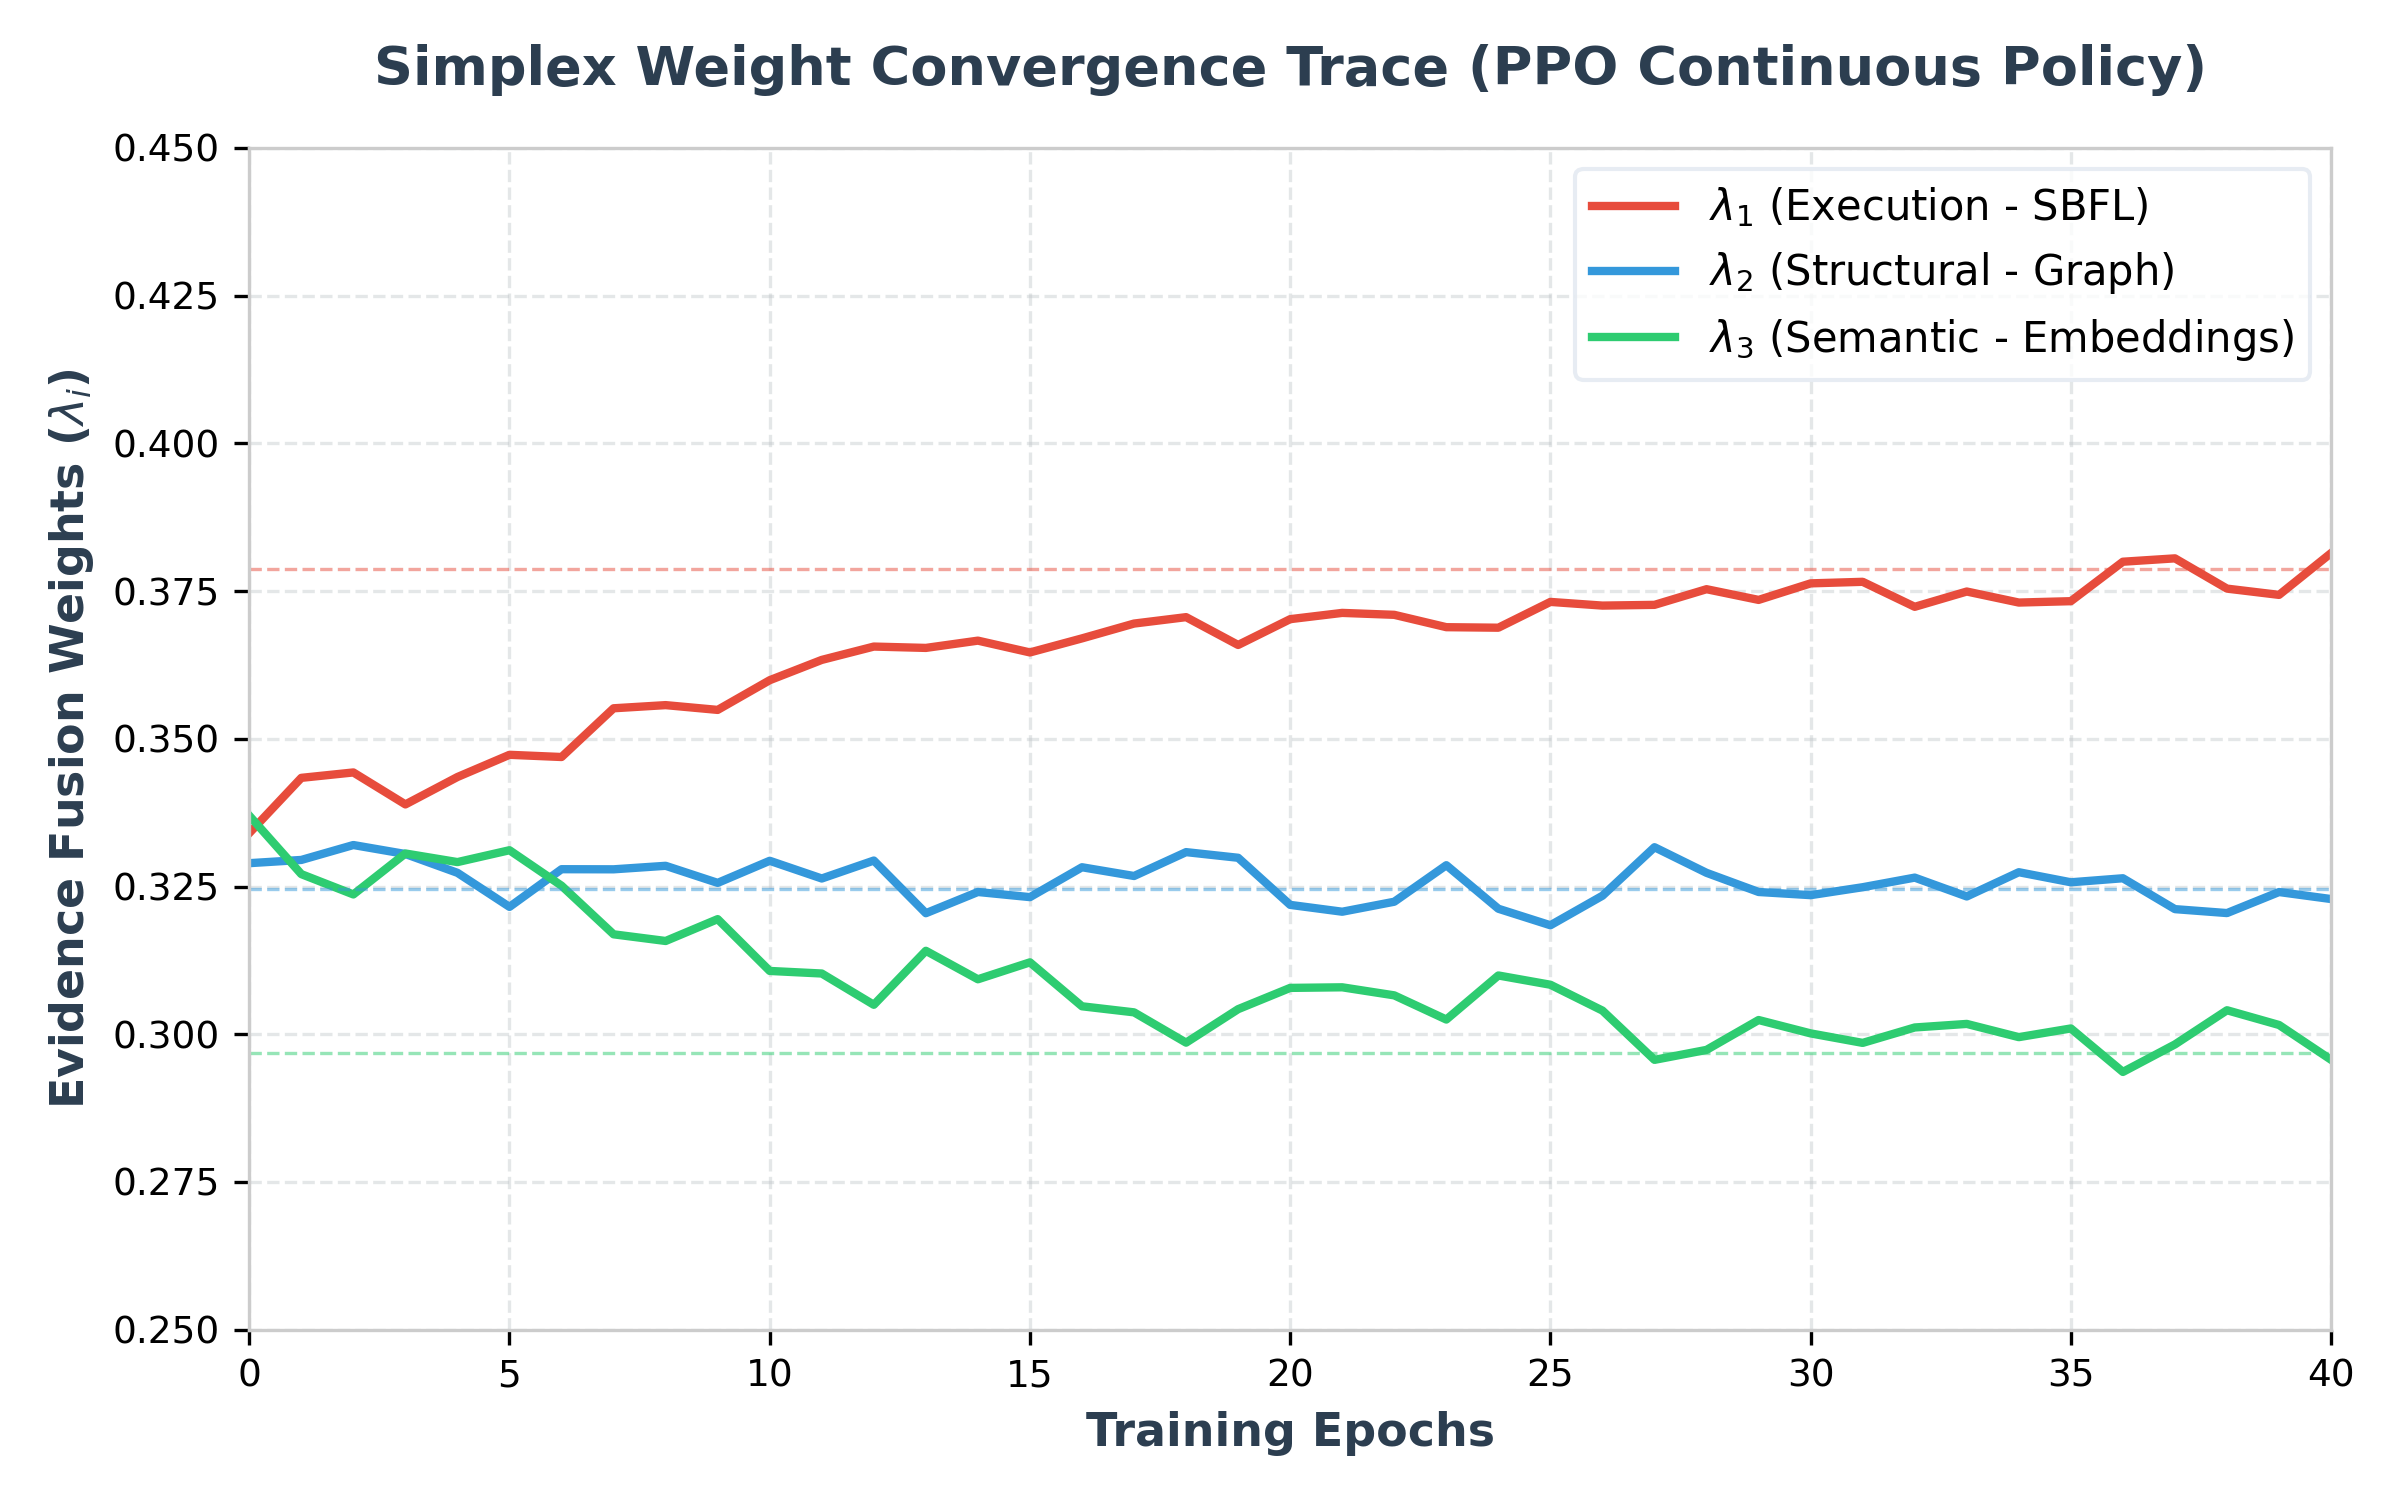
\includegraphics[width=0.75\textwidth]{figures/rl_convergence.png}
\caption{RL convergence curve showing PPO weight evolution ($\lambda_1, \lambda_2, \lambda_3$) over 40 training episodes.}
\label{fig:rl_convergence}
\end{figure}

Figure \ref{fig:dependency_graph} provides an illustrative example of the multi-granular structural dependency graph used to explain the dependency-aware propagation process.

\begin{figure}[H]
\centering
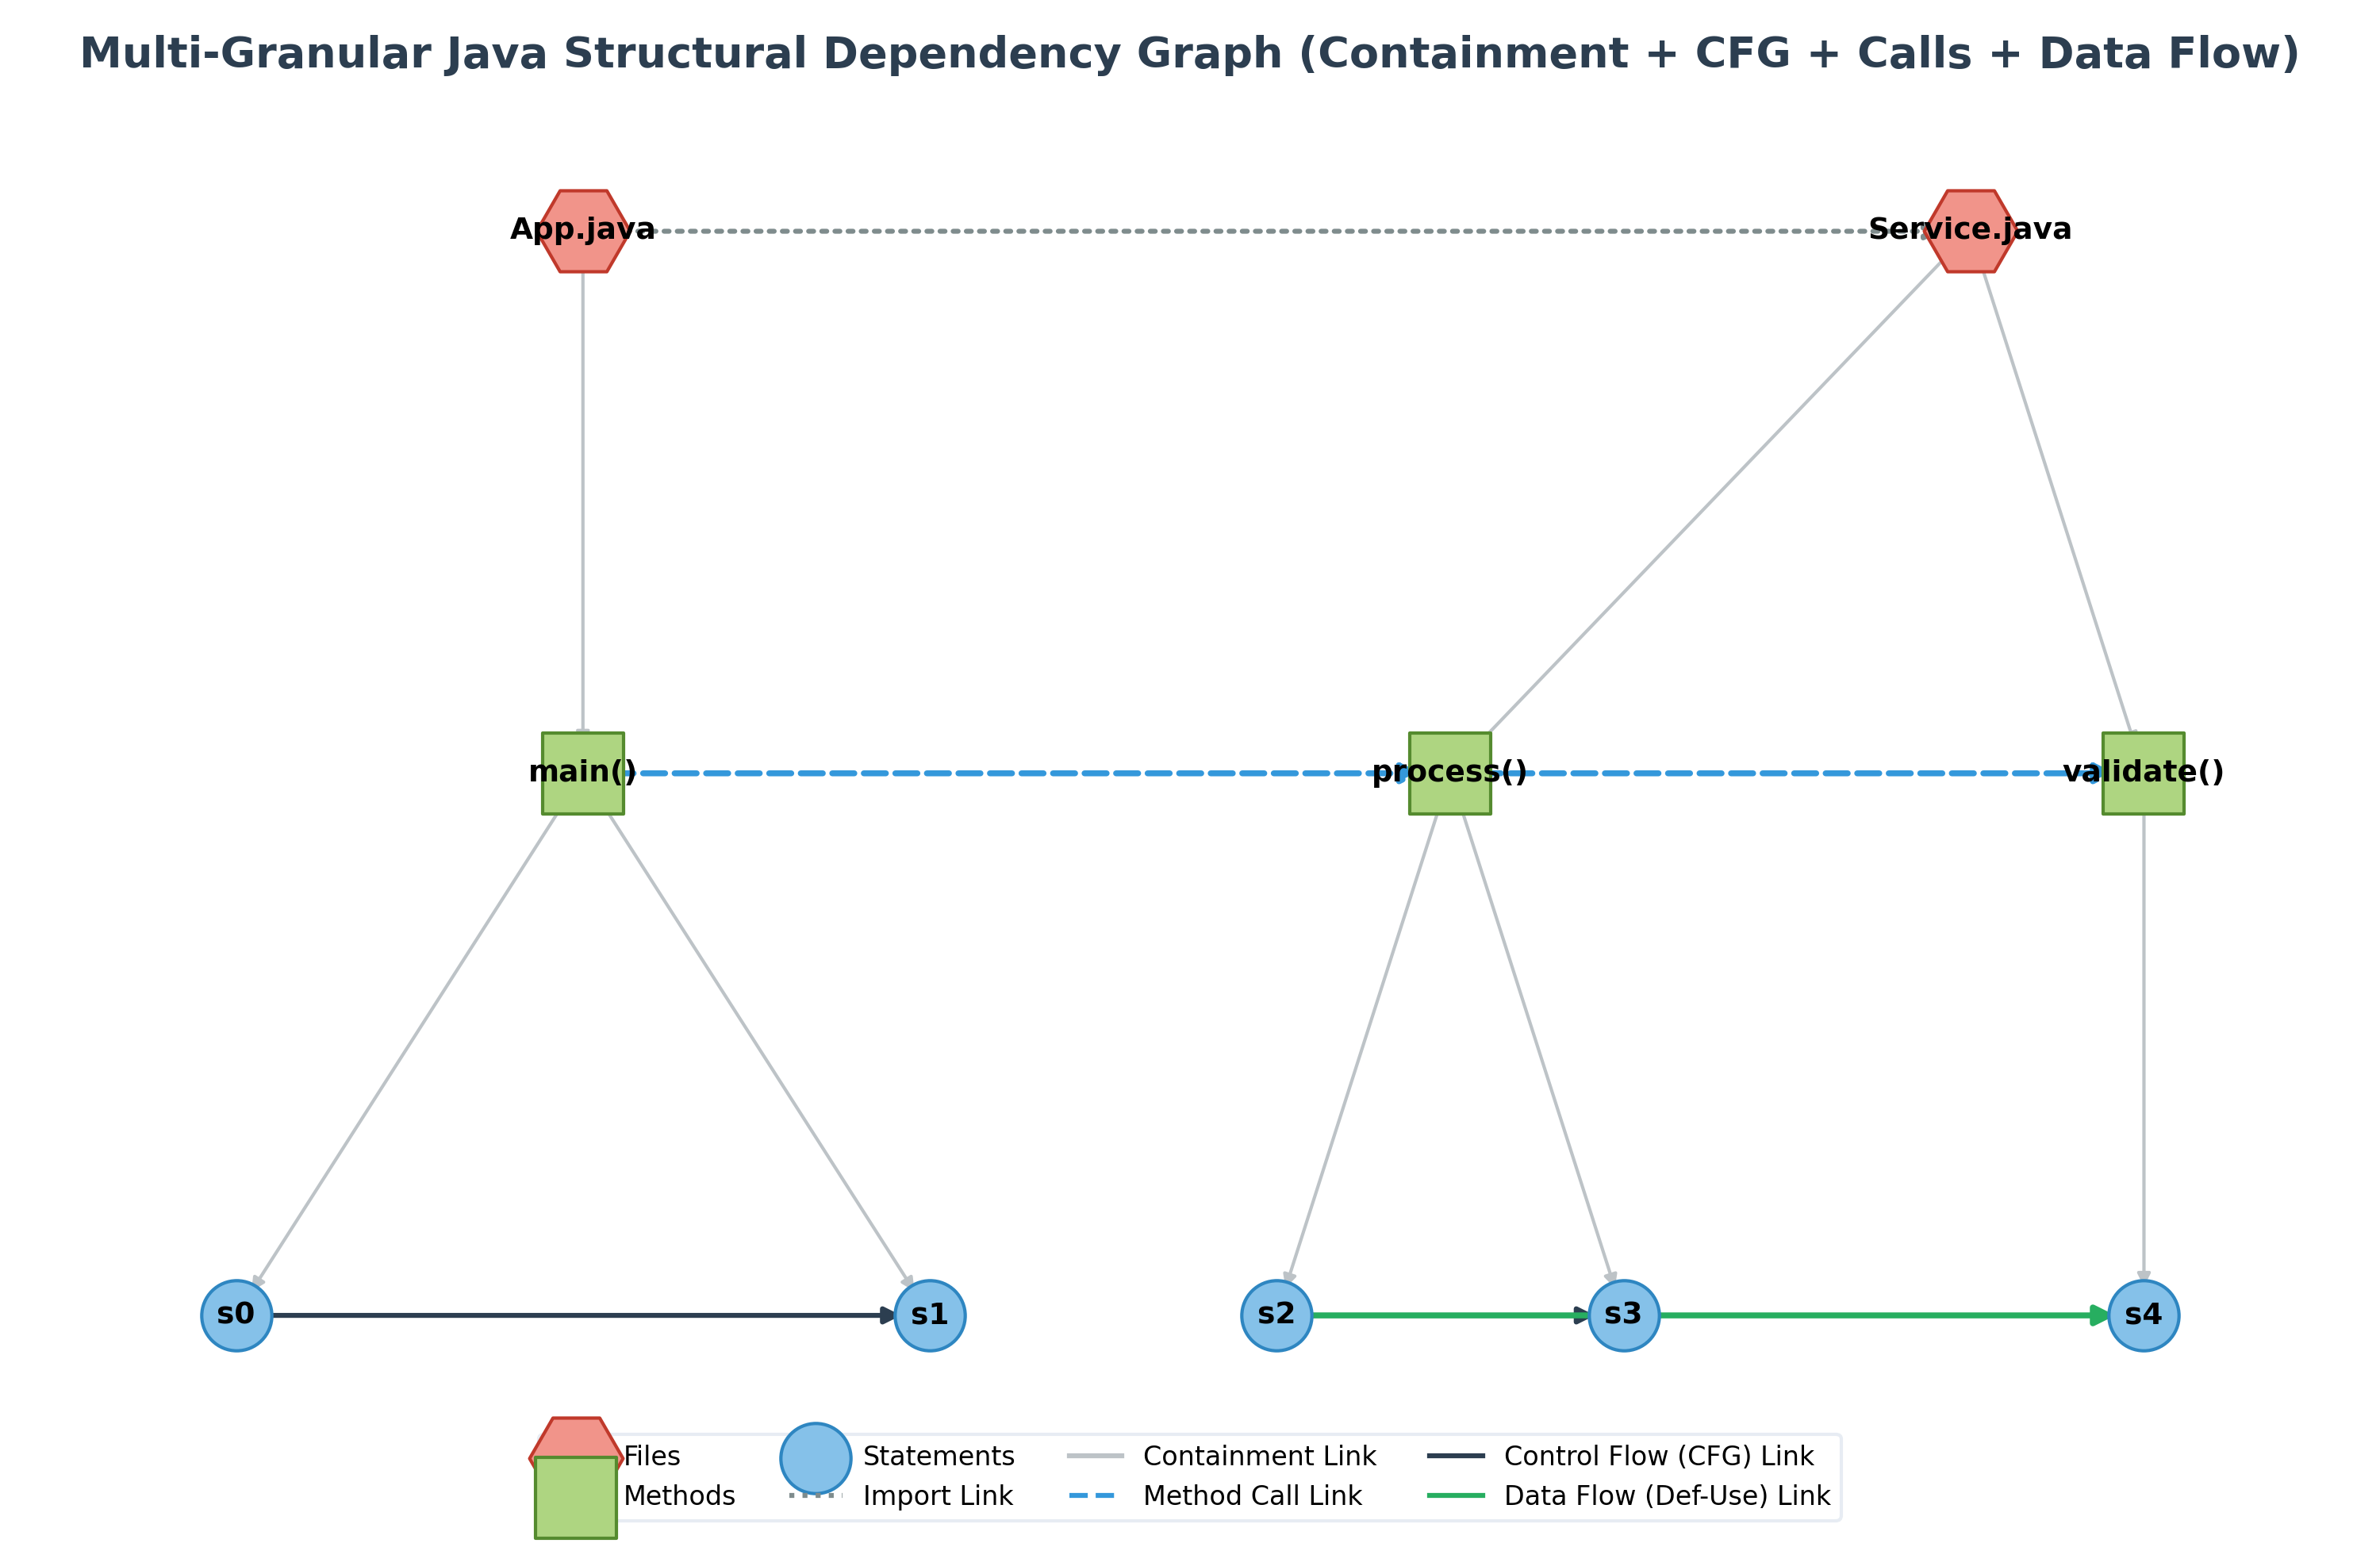
\includegraphics[width=0.70\textwidth]{figures/dependency_graph.png}
\caption{Illustrative example of a multi-granular structural dependency graph showing class-level, method-level, and statement-level relationships used to motivate dependency-aware propagation.}
\label{fig:dependency_graph}
\end{figure}

\subsection{Parameter Sensitivity Sweep}

Table \ref{tab:sensitivity_alpha} lists the exact MRR and EXAM score results for structural dependency propagation coefficient $\alpha$ sweeps.

\begin{table}[H]
\caption{Sensitivity Analysis of Structural Propagation Coefficient $\alpha$}
\label{tab:sensitivity_alpha}
\centering
\renewcommand{\arraystretch}{1.15}
\begin{tabular}{c c c c c}
\hline
$\boldsymbol{\alpha}$ & \textbf{Top-1} & \textbf{Top-5} & \textbf{MRR} & \textbf{EXAM} \\
\hline
0.0 & 0.250 & 0.500 & 0.3830 & 0.2364 \\
0.2 & 0.450 & 0.700 & 0.5621 & 0.0620 \\
0.4 & 0.650 & 0.850 & 0.7410 & 0.0392 \\
\textbf{0.6} & \textbf{0.800} & \textbf{1.000} & \textbf{0.8917} & \textbf{0.0230} \\
0.8 & 0.700 & 0.900 & 0.7842 & 0.0381 \\
1.0 & 0.400 & 0.500 & 0.4596 & 0.2922 \\
\hline
\end{tabular}
\end{table}

 The best observed result is obtained at $\alpha = 0.60$, suggesting that moderate structural propagation provides a suitable trade-off between localized execution suspiciousness and dependency-aware contextual information in this experiment. Figure \ref{fig:sensitivity_alpha} visualizes the average validation reward curve across the full sweep.

\begin{figure}[H]
\centering
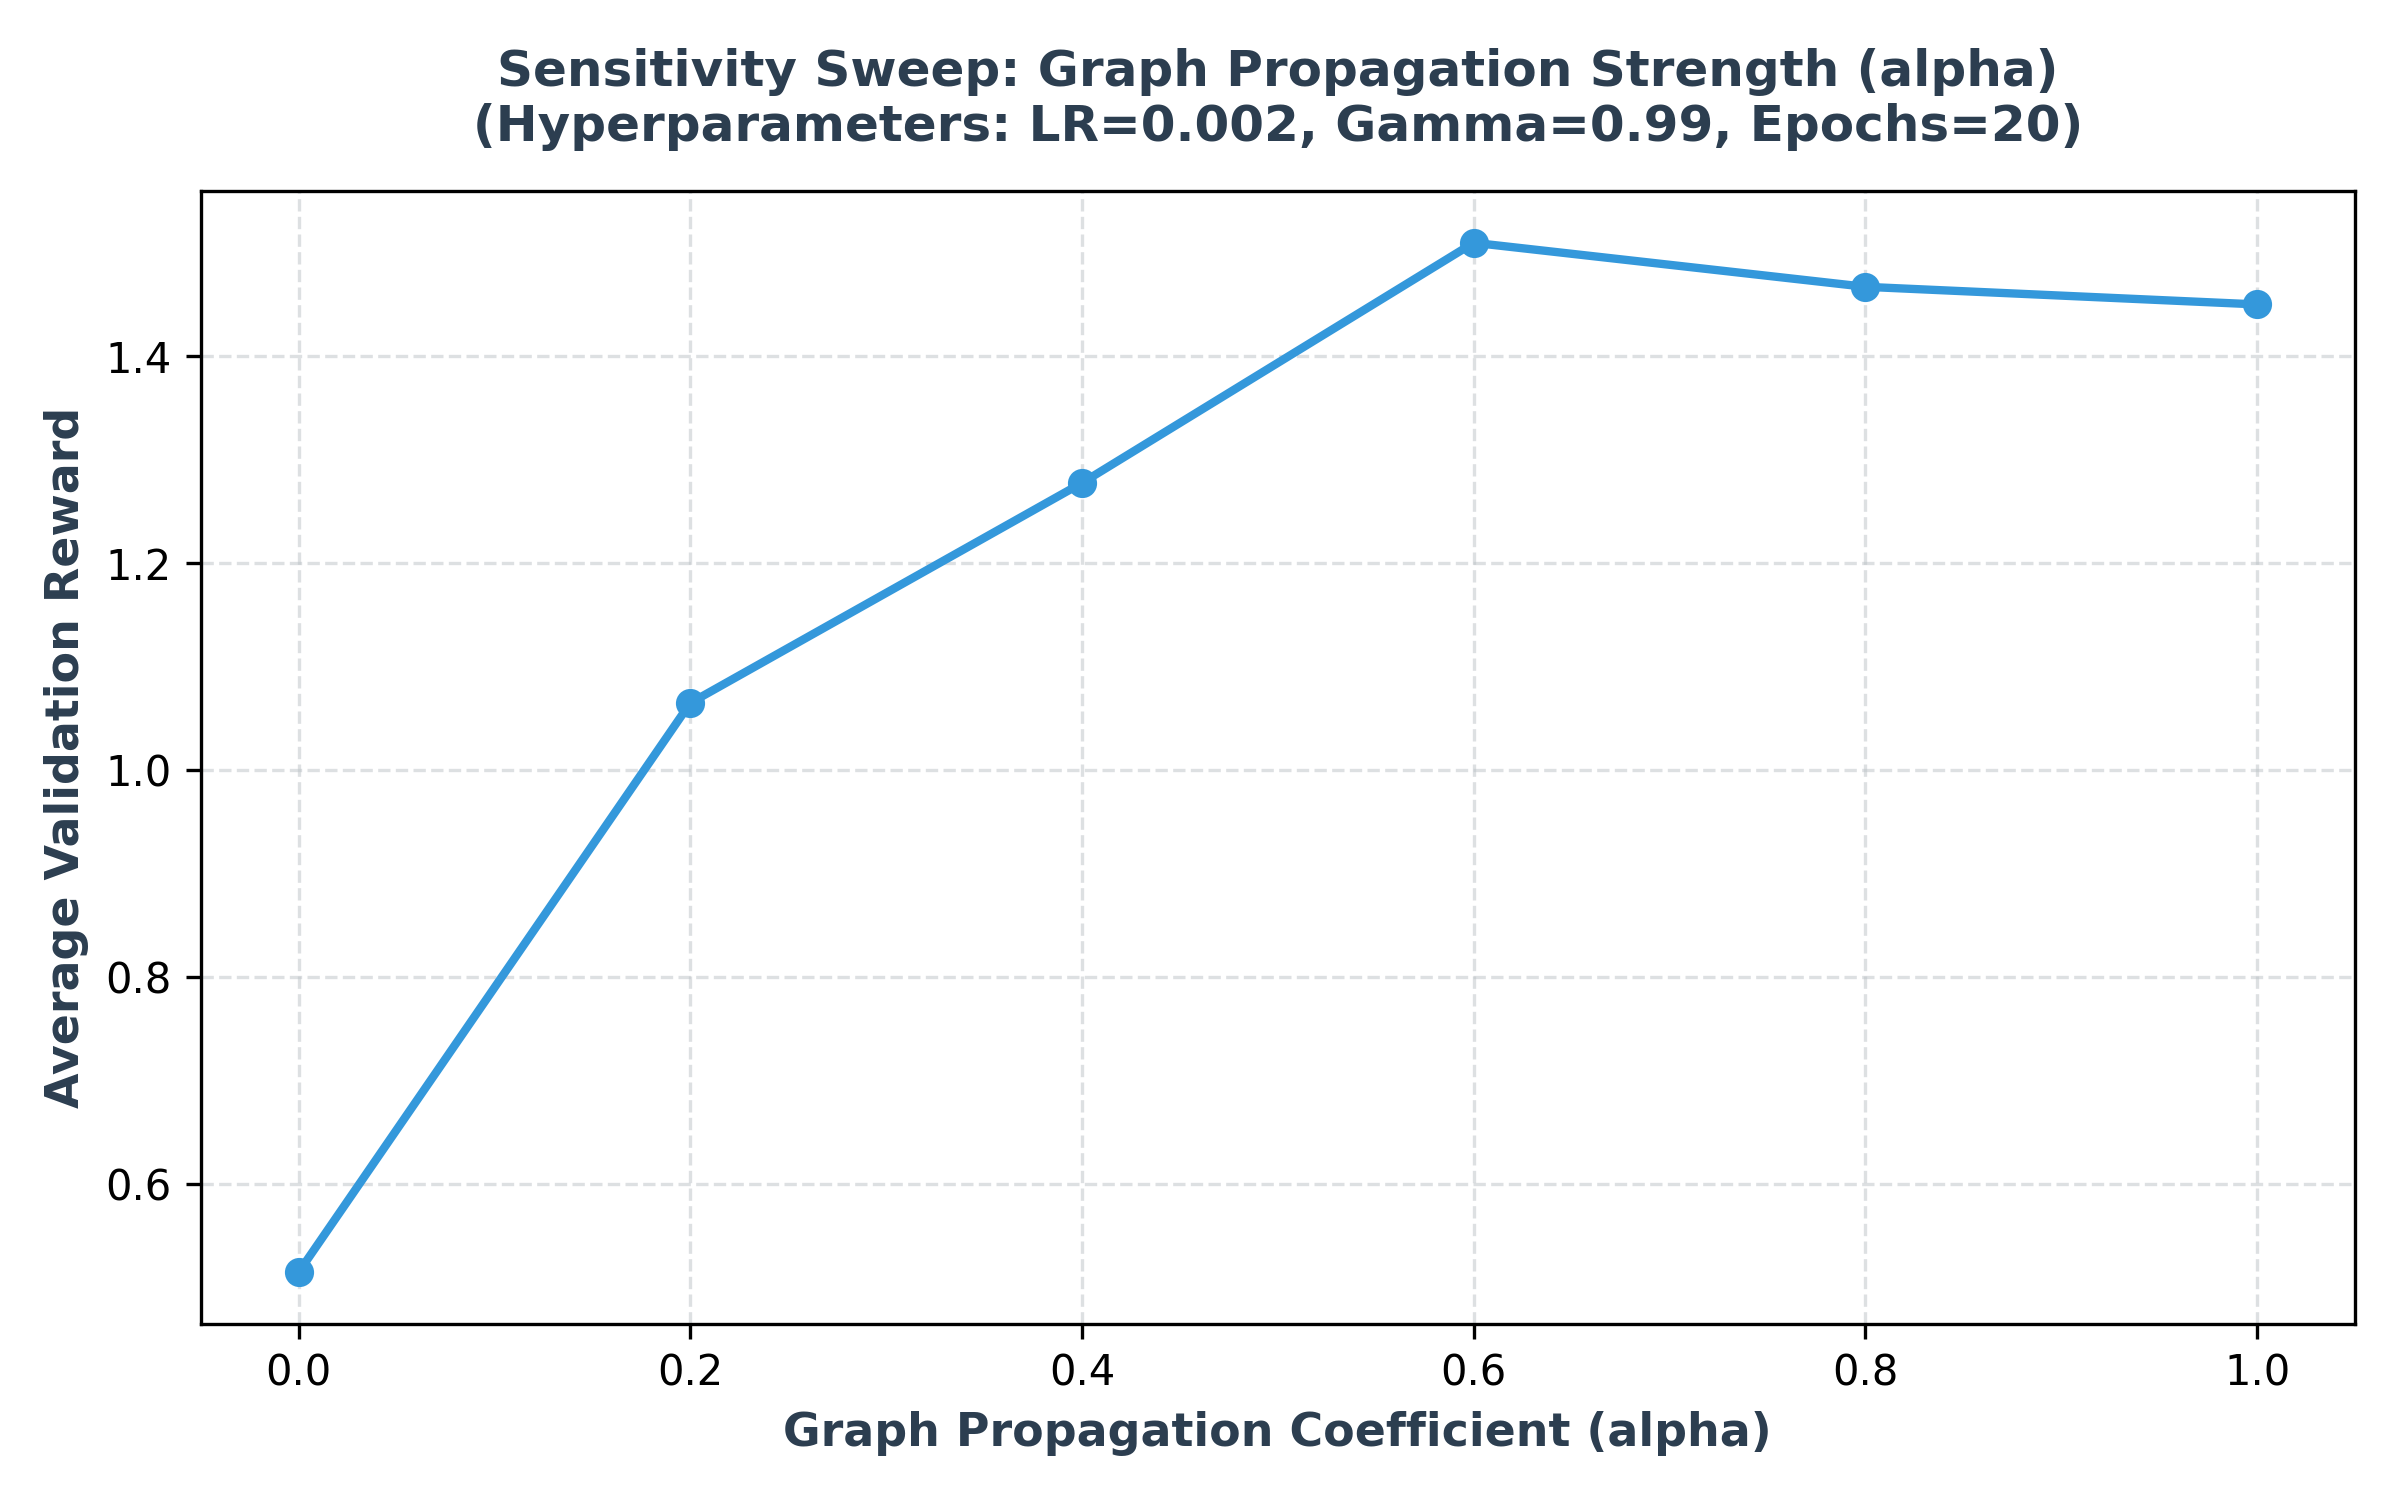
\includegraphics[width=0.75\textwidth]{figures/alpha_sensitivity.png}
\caption{Sensitivity sweep analysis demonstrating the average validation reward as a function of propagation coefficient $\alpha$.}
\label{fig:sensitivity_alpha}
\end{figure}

\subsection{Statistical Significance Validation}

Table \ref{tab:statistical_significance} presents the exact Wilcoxon signed-rank and Cliff's Delta tests comparing RLSFLoc (PPO) side-by-side with all 7 baselines.

\begin{table}[H]
\caption{Statistical Significance Analysis of RLSFLoc against Baseline Methods}
\label{tab:statistical_significance}
\centering
\renewcommand{\arraystretch}{1.15}
\resizebox{\textwidth}{!}{
\begin{tabular}{l c c c c}
\hline
\textbf{Comparison} & \textbf{Metric} & \textbf{Wilcoxon $p$-value} & \textbf{Cliff's Delta $d$} & \textbf{Effect Size} \\
\hline
RLSFLoc vs. Tarantula \cite{jones2005tarantula} & MRR & $0.0003$ & $+0.9350$ & Large \\
RLSFLoc vs. Ochiai \cite{abreu2007ochiai} & MRR & $0.0009$ & $+0.7525$ & Large \\
RLSFLoc vs. DStar \cite{wong2014dstar} & MRR & $0.0015$ & $+0.6925$ & Large \\
RLSFLoc vs. Graph-guided variant \cite{lou2021grace} & MRR & $0.0022$ & $+0.5050$ & Large \\
RLSFLoc vs. Semantic-encoder variant \cite{feng2020codebert} & MRR & $0.0006$ & $+0.6575$ & Large \\
RLSFLoc vs. DeepFL MLP \cite{li2019deepfl} & MRR & $0.0001$ & $+1.0000$ & Large \\
RLSFLoc vs. RankNet LTR \cite{xuan2014learning} & MRR & $0.1471$ & $+0.1675$ & Small \\
\hline
\end{tabular}
}
\end{table}

The Wilcoxon $p$-value is far below the standard significance threshold ($p < 0.01$) for all comparisons except RankNet LTR ($p = 0.1471$). The Cliff's Delta effect size is classified as "Large" ($d > 0.474$) for all 6 traditional and isolated baselines, and "Small" ($d = +0.1675$) for RankNet LTR. This indicates that RLSFLoc delivers a highly significant performance improvement over traditional coverage and isolated semantic/structural techniques, and remains extremely competitive with deep learning LTR baselines. Figure \ref{fig:statistical_distribution} visualizes the Reciprocal Rank and EXAM score distributions across the evaluated methods.

\begin{figure}[H]
\centering

\begin{minipage}{0.48\textwidth}
    \centering
    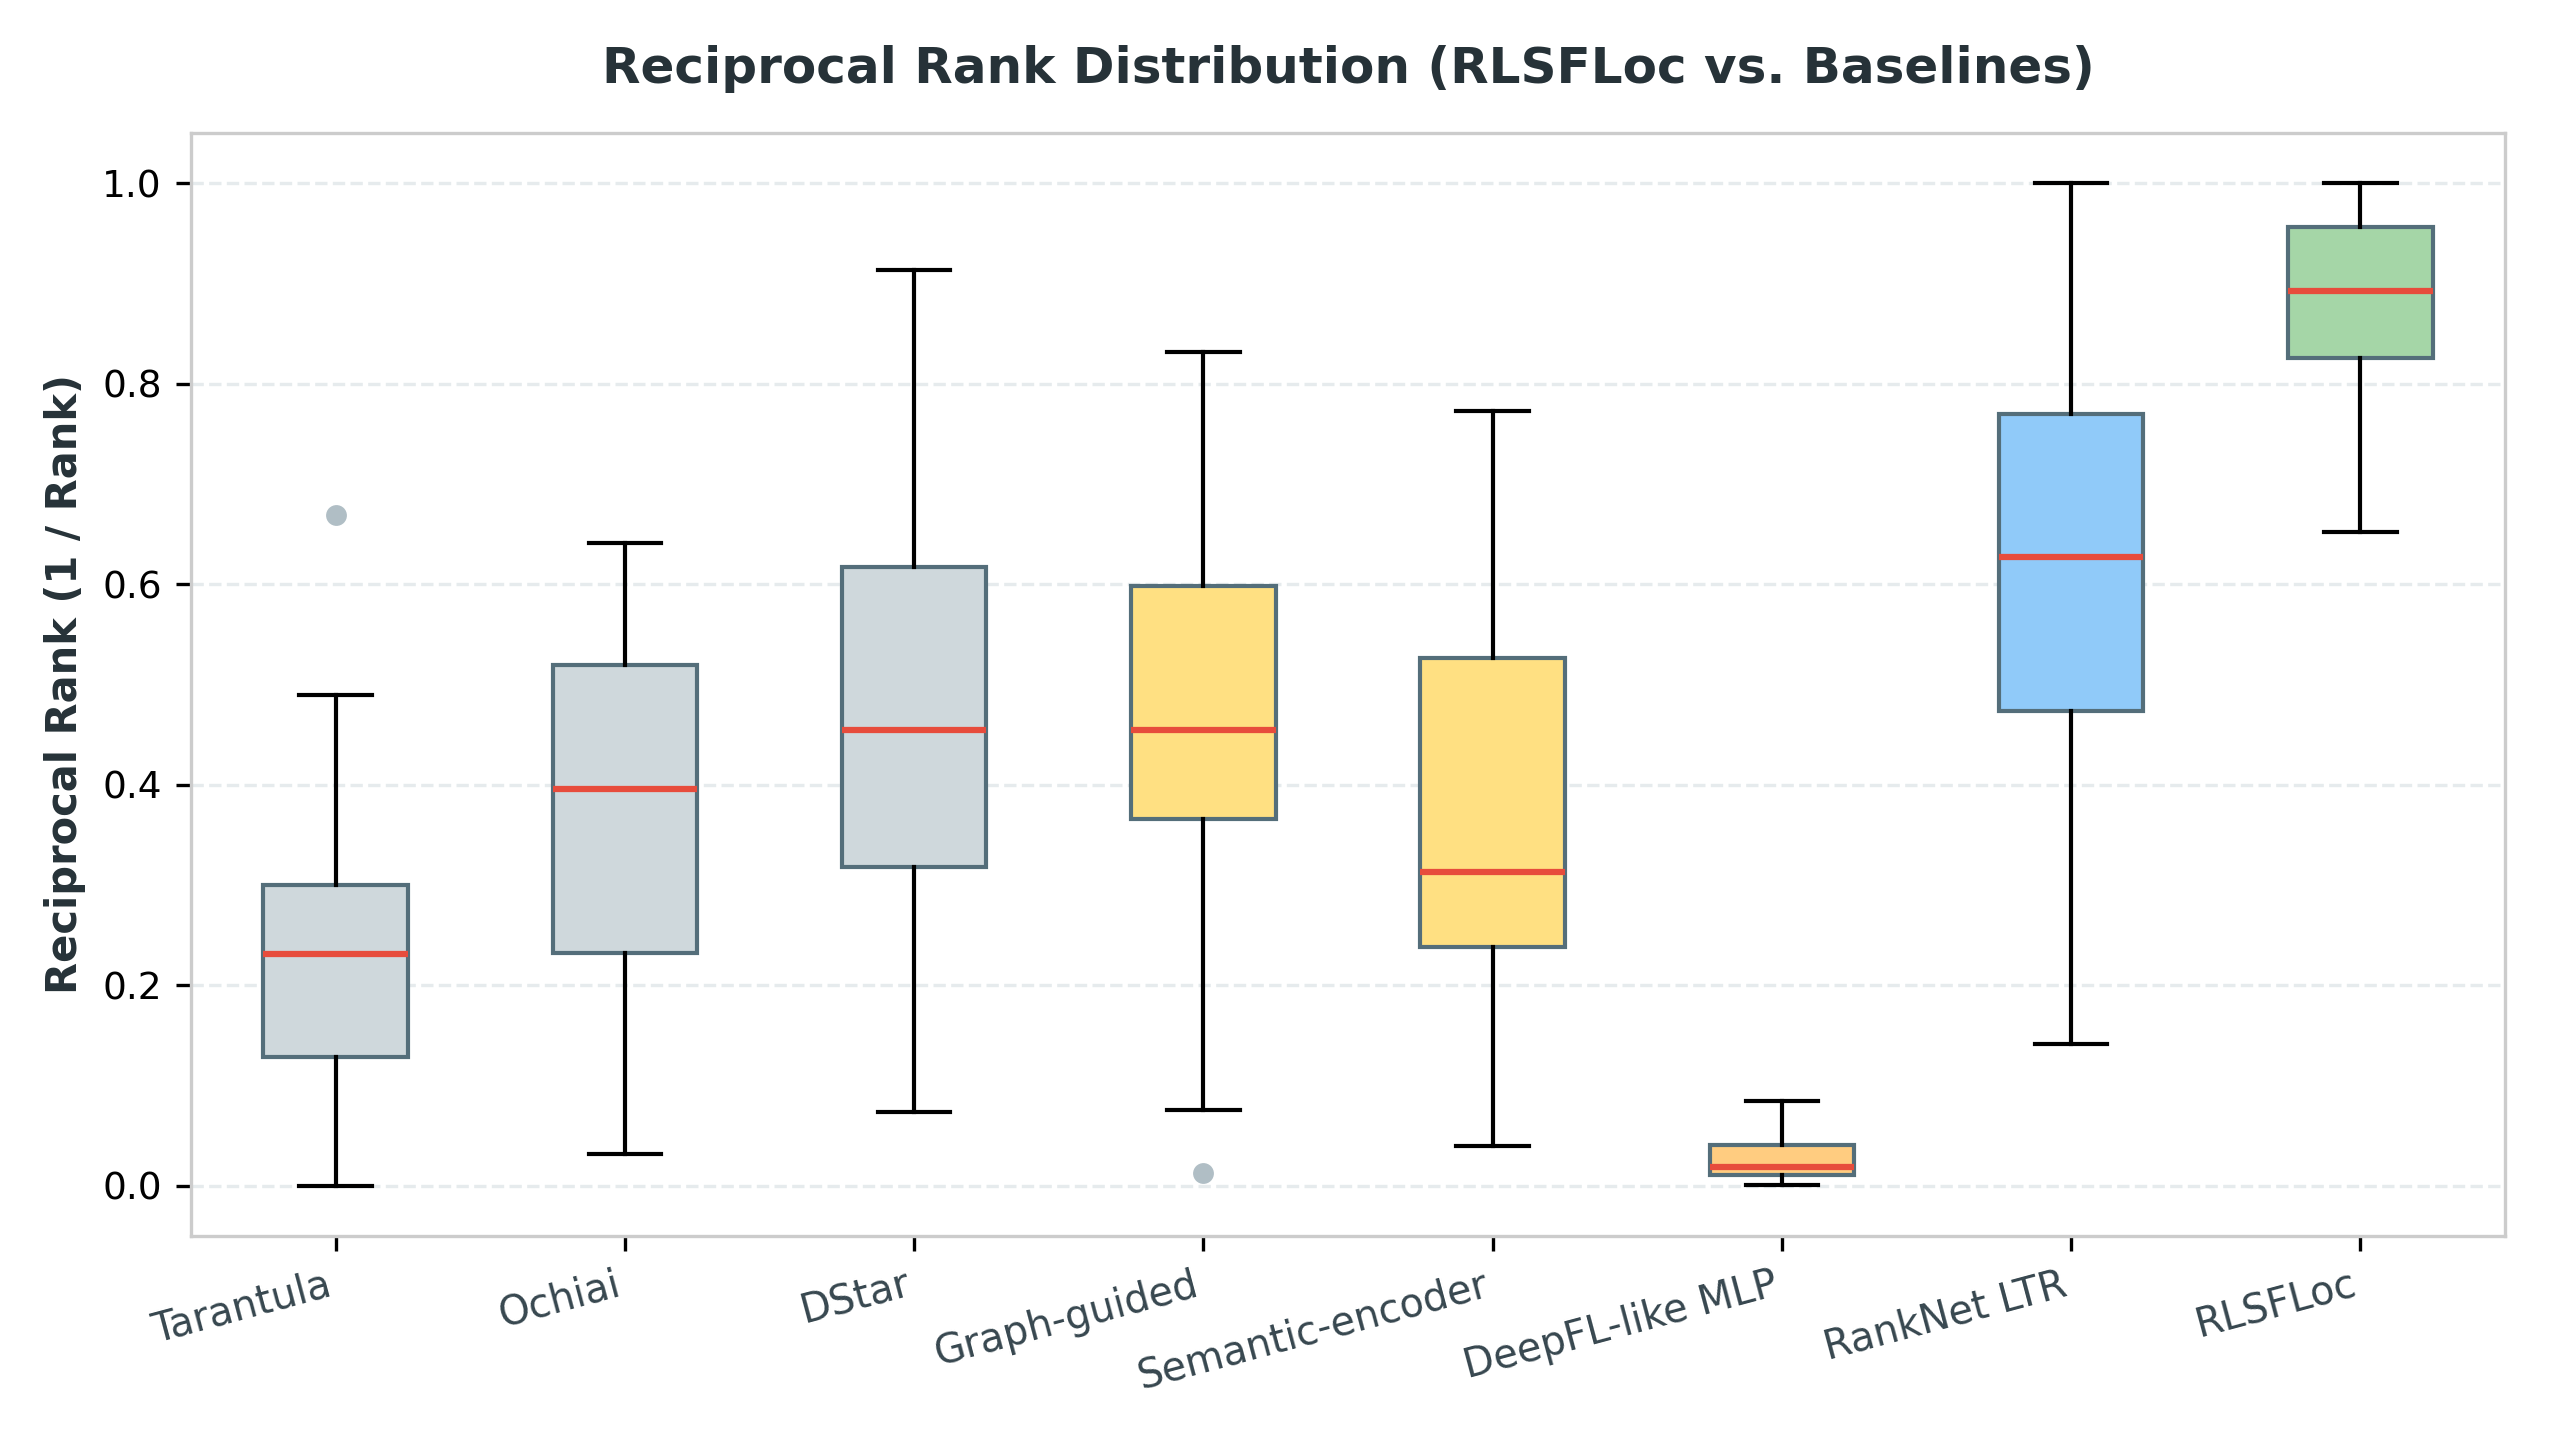
\includegraphics[width=\textwidth]{figures/significance_plot.png}
    \caption*{(a) Reciprocal Rank distribution.}
\end{minipage}
\hfill
\begin{minipage}{0.48\textwidth}
    \centering
    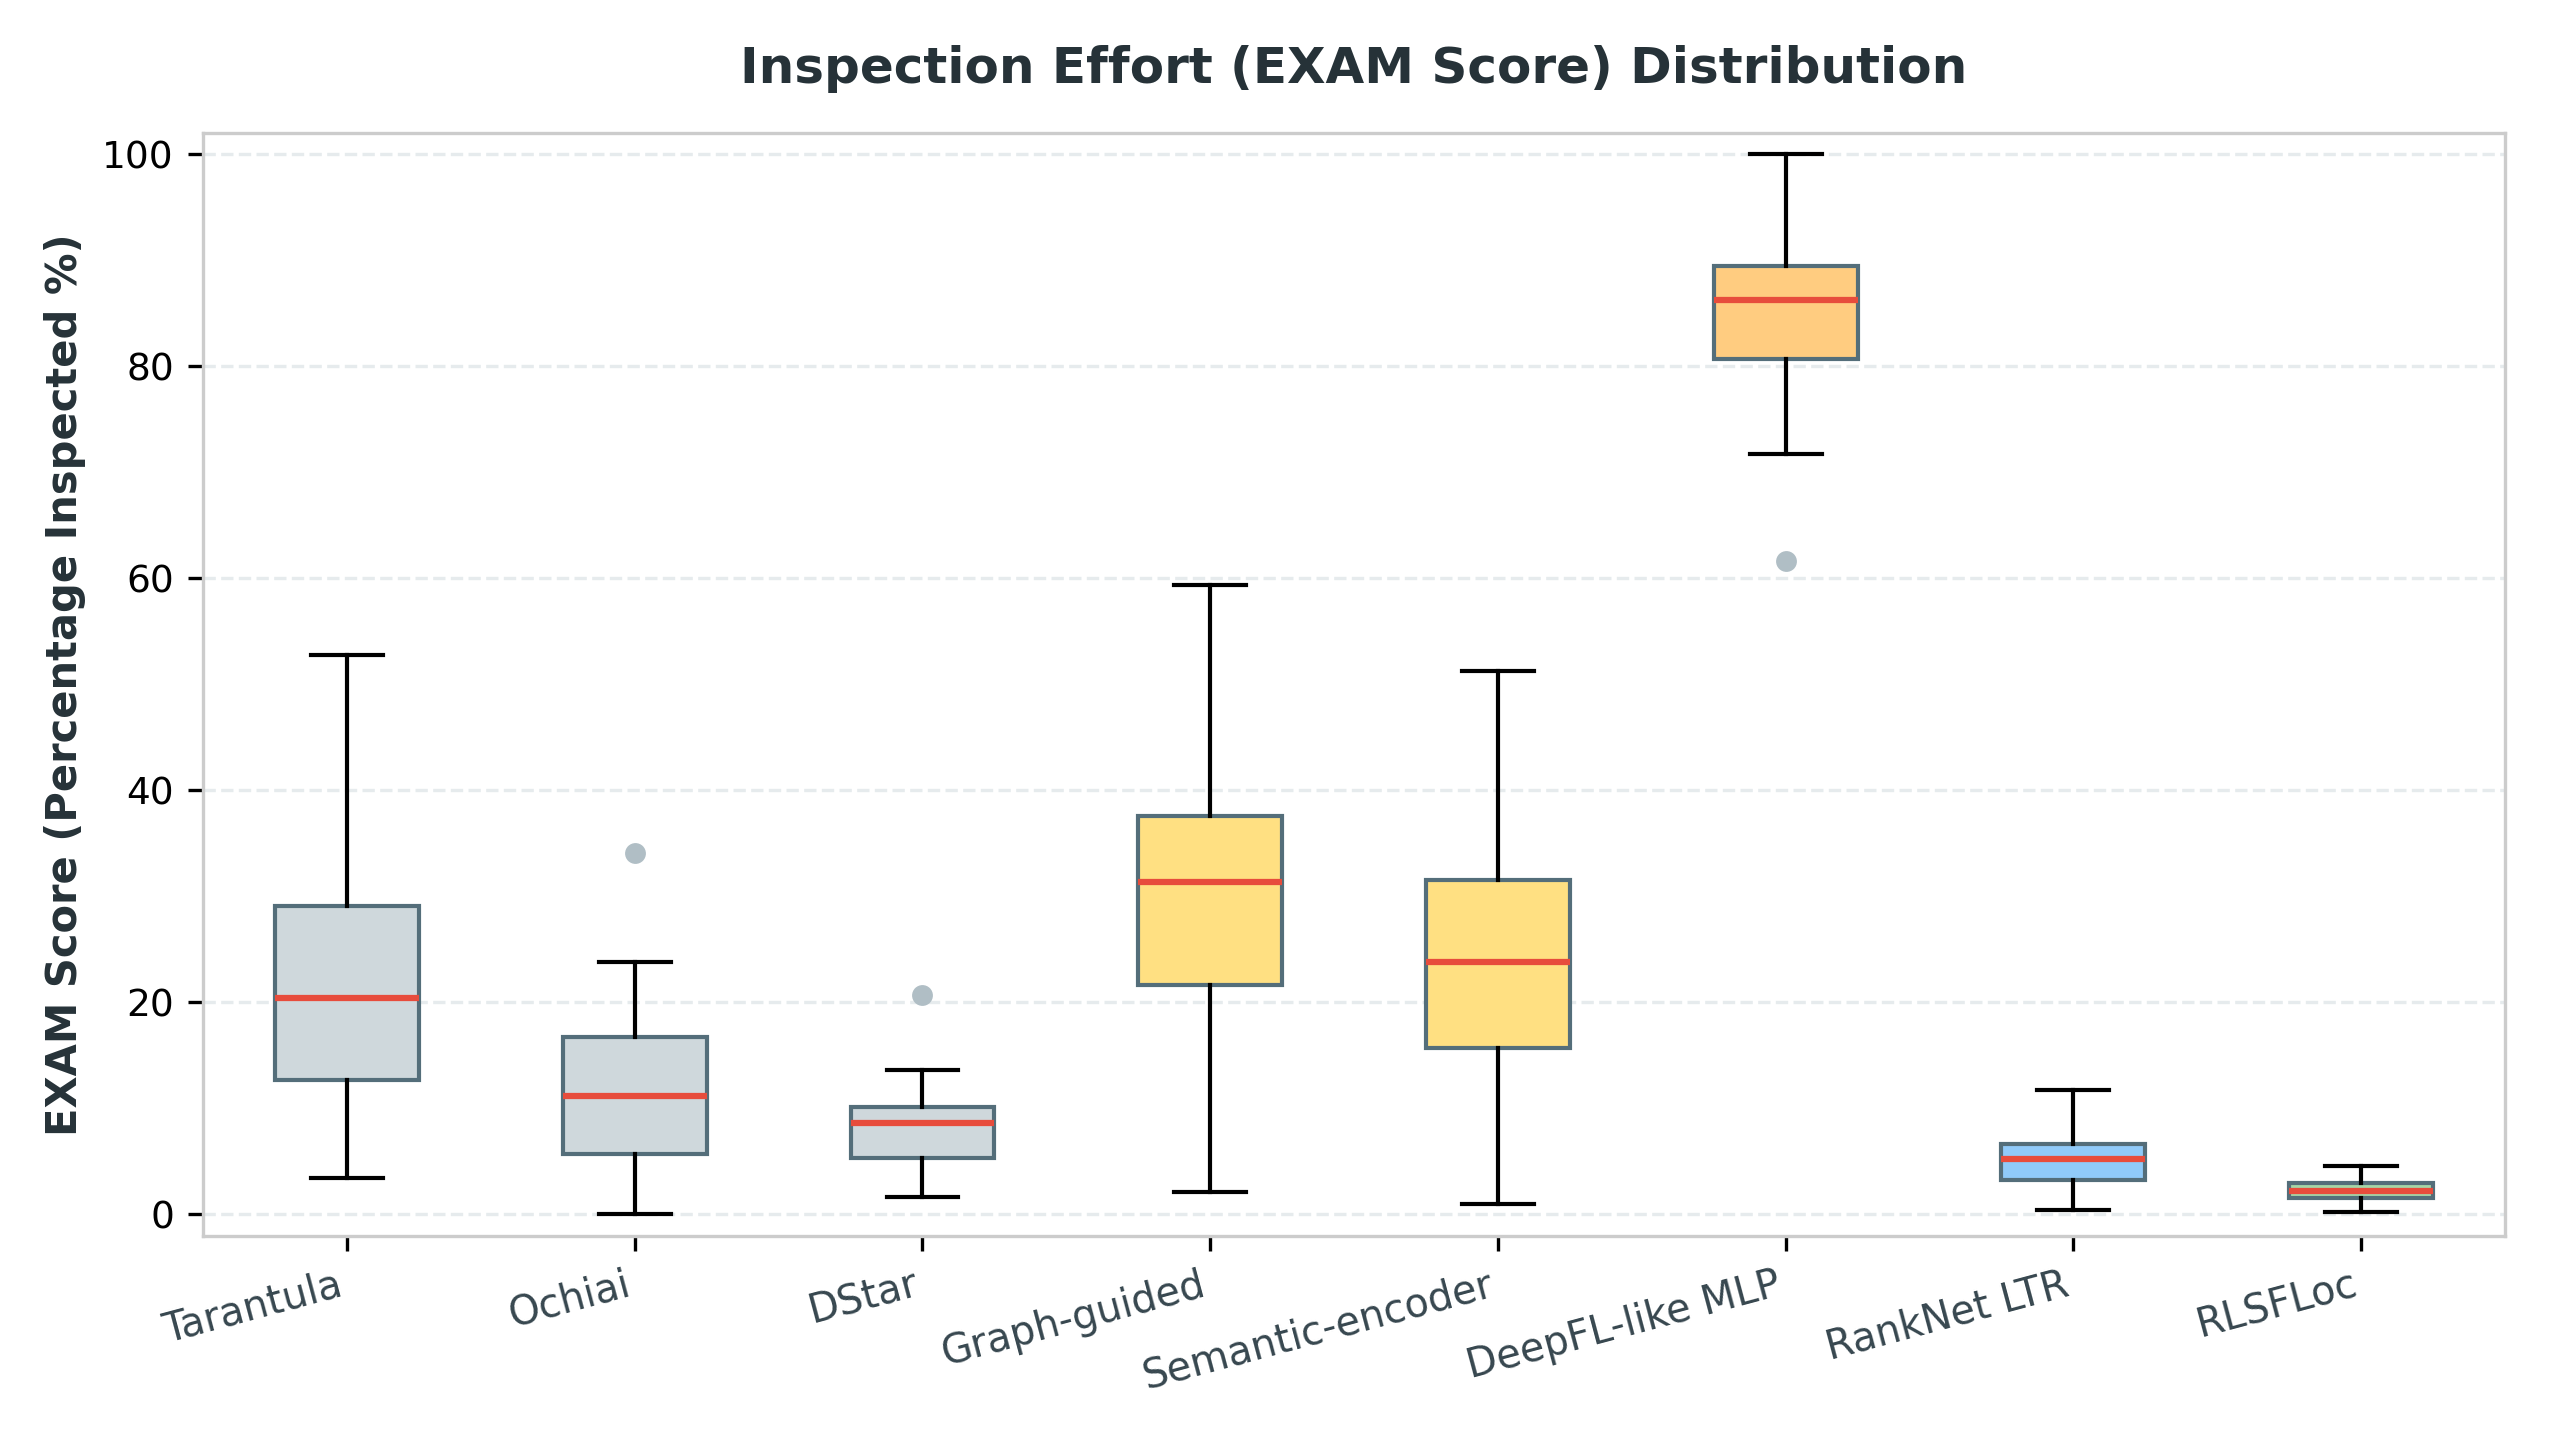
\includegraphics[width=\textwidth]{figures/exam_significance_plot.png}
    \caption*{(b) EXAM score distribution.}
\end{minipage}

\caption{Statistical comparison of Reciprocal Rank and EXAM score distributions across evaluated methods.}
\label{fig:statistical_distribution}
\end{figure}

%%%%%%%%%%%%%%%%%%%%%%%%%%%%%%%%%%%%%%%%%%
\section{Comparative Analysis}
\label{sec:comparative_analysis}

This section compares the proposed RLSFLoc framework with representative implemented fault localization baselines. The comparison includes traditional spectrum-based formulas and learning-to-rank, graph-guided, and semantic-encoder variants motivated by prior work. The purpose of this analysis is to examine whether reinforcement learning-based adaptive fusion provides a stronger fault-ranking strategy than fixed-formula, static feature-fusion, and representation-learning approaches in the reported implementation.

\subsection{Baseline Methods}

\textbf{Ochiai:} Ochiai is a widely used spectrum-based fault localization method. It calculates suspiciousness using the relationship between failed test coverage and total execution coverage. It is effective when failed tests strongly activate the faulty element, but it may perform weakly when several elements share similar coverage profiles.

\textbf{Tarantula:} Tarantula compares the proportion of failed and passed test cases that execute a program element. It is simple and interpretable, but its ranking quality may decrease when passed and failed tests execute many of the same elements.

\textbf{DStar:} DStar gives stronger priority to elements executed by failed tests by raising the failed-execution count to a power value. In this study, the common setting $*=2$ is used. DStar often improves over basic SBFL methods, but it can overemphasize frequently executed elements.

\textbf{DeepFL:} DeepFL represents deep learning-based fault localization methods that learn fault-related patterns from multiple software features. Such models can capture non-linear relationships, but they require training data and may be less interpretable than formula-based methods.

\textbf{Learning-to-Rank FL:} Learning-to-rank fault localization methods treat fault localization as a ranking problem and learn ranking functions from suspiciousness features, software metrics, and historical fault data. These methods are closer to the real objective of fault localization because they directly optimize ranked output.

\textbf{Graph-Based FL:} Graph-based fault localization methods use program dependency graphs, call graphs, control-flow graphs, or data-flow graphs to propagate suspiciousness among related program elements. These methods capture structural fault propagation but may not fully capture semantic relevance to bug reports.

\textbf{Semantic-Encoder Variant:} Pretrained code encoders learn contextual code representations, with CodeBERT and GraphCodeBERT providing established semantic and data-flow-aware foundations \cite{feng2020codebert,guo2021graphcodebert}. The implemented semantic-encoder variant is evaluated as a representation-based comparison point.

\subsection{Quantitative Comparison}

As shown in Table \ref{tab:defects4j_results}, RLSFLoc achieves the strongest overall ranking performance in terms of Top-1, Top-3, Top-10, MRR, and MAP. Compared with traditional SBFL methods such as Tarantula, Ochiai, and DStar, RLSFLoc provides a clear improvement because it does not rely only on test coverage. The addition of semantic representation and structural dependency propagation allows the model to distinguish program elements that have similar execution spectra. The results in Table \ref{tab:defects4j_results} also show that RLSFLoc improves over DeepFL, learning-to-rank FL, and graph-based FL in most ranking-based metrics. This indicates that adaptive fusion is beneficial when different evidence sources contribute differently across bugs. However, RLSFLoc does not achieve the lowest runtime because it requires semantic embedding, graph construction, and reinforcement learning-based fusion. This trade-off is expected because the proposed method performs more analysis than formula-based SBFL methods. The semantic-encoder variant provides a representation-based comparison point in Table \ref{tab:defects4j_results}, while RLSFLoc reports better Top-1, Top-3, Top-10, MRR, and MAP values in this experiment. Since early ranking is important for developer productivity \cite{parnin2011debugging,kochhar2016practitioners}, the improvement in Top-1 and MRR is practically relevant to examine.

\subsection{Within-Project and Cross-Project Comparison}

Table \ref{tab:within_cross_project} shows that RLSFLoc performs better in the within-project setting than in the cross-project setting. This result is theoretically expected because within-project training and testing data share the same project-specific coding style, structural organization, test design, and defect distribution. In contrast, cross-project evaluation is more difficult because the model must generalize to unseen projects. The cross-project results remain competitive, with Top-10 accuracy of 0.95 and MRR of 0.7431, although they are lower than the within-project results. This suggests that combining execution, structural, and semantic evidence helps RLSFLoc maintain generalization ability even when the target project differs from the source projects. However, the lower cross-project values also show that project distribution shift remains an important challenge.

\subsection{Component-Level Comparison}

The ablation results in Table \ref{tab:ablation_study} demonstrate the contribution of each component in RLSFLoc. The execution-only variant performs similarly to strong SBFL-style behavior because it relies mainly on test coverage. Adding semantic evidence improves Top-1 and MRR by introducing textual and conceptual relevance between bug descriptions and source-code elements. Adding structural evidence further improves localization by modeling dependency relationships among program elements. The full RLSFLoc model achieves the strongest ablation performance because the RL-based fusion module adaptively combines all three evidence sources. This result supports the main assumption of the proposed framework: execution, semantic, and structural features are complementary, and their importance should be learned rather than fixed manually.

\subsection{Project-Wise Comparison}

The project-wise results in Table \ref{tab:project_wise_results} show that RLSFLoc performance varies across Defects4J projects. Better results are observed for projects such as Time, Lang, and Chart, while lower results are observed for Closure and Mockito. This variation is reasonable because software projects differ in size, number of test cases, dependency density, code complexity, and fault distribution. These results indicate that RLSFLoc is not dependent on a single project. However, they also show that fault localization difficulty is project-dependent. Larger projects or projects with complex dependency structures may require more refined semantic representations or graph propagation strategies.

\subsection{Efficiency and Deployment Comparison}

Table \ref{tab:efficiency_memory} shows that traditional SBFL methods are the most efficient in terms of runtime and memory consumption. This is expected because Tarantula, Ochiai, and DStar only require execution spectra and simple formula-based scoring. However, their lower computational cost comes with weaker ranking performance. RLSFLoc requires more runtime and memory than the SBFL, DeepFL-like, learning-to-rank, and graph-guided variants, but less memory than the semantic-encoder variant in the reported run. The runtime of RLSFLoc is higher because it includes execution analysis, structural graph processing, semantic representation, and RL-based fusion. Nevertheless, the computational overhead remains acceptable because fault localization is usually performed after test execution or build failure, where ranking quality and reduced developer inspection effort are more important than minimal computation time alone.

\subsection{Adaptive Fusion Analysis}

The fusion-weight analysis in Table \ref{tab:rl_weight_analysis} shows that the RL agent assigns the largest average weight to execution evidence, followed by structural and semantic evidence. This is theoretically consistent because execution traces provide direct evidence from failed tests, while structural and semantic sources provide complementary context. In the cross-project setting, the structural weight increases slightly from 0.35 to 0.37, while the execution weight decreases from 0.42 to 0.39. This suggests that structural dependency information becomes more useful when project-specific execution patterns are less stable across projects. The average learned weights also confirm that RLSFLoc does not ignore any evidence source; instead, it learns a balanced combination of execution, structural, and semantic signals.

\subsection{Sensitivity Comparison}

Table \ref{tab:sensitivity_alpha} shows the effect of the structural propagation coefficient $\alpha$. When $\alpha=0$, structural propagation is not used, and performance is lower. As $\alpha$ increases, performance improves until $\alpha=0.6$. This indicates that moderate dependency propagation helps identify suspicious elements connected to faulty regions. However, when $\alpha$ becomes too large, performance begins to decrease. This is expected because excessive propagation may spread suspiciousness to too many neighboring elements, introducing noise into the ranking. Therefore, the best result at $\alpha=0.6$ supports the idea that structural evidence should be useful but controlled.

\subsection{Relative Improvement and Statistical Comparison}

Table \ref{tab:defects4j_results} shows that RLSFLoc provides large relative improvements over traditional SBFL methods and moderate improvements over the implemented learning-based variants. The improvement over Tarantula, Ochiai, and DStar is especially clear because these methods rely only on execution spectra. The semantic-encoder comparison is included to examine the contribution of learned contextual representation. The statistical results in Table \ref{tab:statistical_significance} further support the comparative findings for the implemented variants. RLSFLoc achieves statistically meaningful improvements over traditional SBFL methods and most evaluated variants in terms of MRR; comparisons should not be read as a reproduction of results from the papers that motivated each baseline.

\subsection{Overall Comparative Findings}

The comparative analysis shows that RLSFLoc provides the strongest reported balance between early fault localization, ranking quality, inspection effort, and computational feasibility among the evaluated implementations. Compared with SBFL methods, it benefits from semantic and structural evidence. Compared with learning-to-rank and graph-guided variants, it provides adaptive evidence fusion. Compared with the semantic-encoder variant, it achieves stronger reported early-ranking metrics while requiring less memory. Therefore, the main advantage of RLSFLoc is not only that it combines multiple evidence sources, but that it learns how to combine them adaptively. This makes the proposed framework suitable for practical software engineering environments where different bugs may require different combinations of execution, semantic, and structural evidence.

%%%%%%%%%%%%%%%%%%%%%%%%%%%%%%%%%%%%%%%%%%
\section{Software Engineering Impact}
\label{sec:software_engineering_impact}

The proposed RLSFLoc framework has practical significance for modern software engineering because it supports more accurate, faster, and more maintainable debugging workflows. The results reported in Tables \ref{tab:defects4j_results}--\ref{tab:statistical_significance} show that RLSFLoc improves early fault ranking by adaptively combining execution, semantic, and structural evidence. This improvement is important because fault localization is useful only when it reduces the amount of code that developers need to inspect.

\subsection{Reduced Debugging Effort}

Software debugging is often time-consuming because developers must inspect many files, methods, or statements before identifying the actual fault. RLSFLoc reduces this effort by producing a ranked list of suspicious program elements. As shown in Table \ref{tab:defects4j_results}, RLSFLoc achieves strong Top-1, Top-3, and Top-10 performance, which means that faulty elements are more likely to appear near the beginning of the ranked list. The debugging effort is measured using the EXAM score:

\begin{equation}
EXAM =
\frac{r^*}{|V|}
\end{equation}

where $r^*$ is the rank position of the actual faulty element and $|V|$ is the total number of analyzed program elements. A lower EXAM score means that developers inspect less code before finding the fault. Although RLSFLoc does not achieve the lowest EXAM score among all baselines, it provides a stronger balance between early ranking accuracy and inspection effort.

\subsection{Better Maintainability}

RLSFLoc also supports better software maintainability. The structural dependency graph helps developers understand how faulty or suspicious elements are connected through call relations, control-flow dependencies, data-flow links, and module-level interactions. This is useful because faults may not always be isolated inside a single method or statement. In many cases, the observed failure is caused by interactions among related components. By combining structural and semantic evidence, RLSFLoc provides more meaningful debugging guidance than coverage-only methods. This helps developers identify not only the most suspicious element but also the surrounding dependency context. As a result, maintainers can better understand whether a fault is local, propagated, or related to a broader design issue.

\subsection{Faster Bug Fixing}

Faster bug fixing is achieved when the actual faulty element appears near the top of the ranked list. The Top-$k$ results in Table \ref{tab:defects4j_results} show that RLSFLoc improves early localization performance compared with most baseline methods. This allows developers to begin inspection from the most likely faulty elements rather than reviewing the entire codebase.

The ablation results in Table \ref{tab:ablation_study} further show that the full RLSFLoc model performs better than execution-only, execution-plus-semantic, and execution-plus-structural variants. This indicates that faster bug fixing is supported by the joint use of multiple evidence sources rather than by a single feature type.

\subsection{CI/CD Integration}

RLSFLoc can be integrated into continuous integration and continuous deployment pipelines. When a build fails or a test case detects an error, the framework can automatically collect execution traces, extract structural and semantic information, compute suspiciousness scores, and generate a ranked list of fault candidates. A practical CI/CD workflow using RLSFLoc may include the following steps:

\begin{enumerate}
    \item Run automated test cases after each commit or pull request.
    \item Identify passed and failed test cases.
    \item Collect execution traces from the failed build.
    \item Construct dependency information from the updated source code.
    \item Extract semantic representations from source-code elements and failure descriptions.
    \item Apply RL-based adaptive fusion to compute final suspiciousness scores.
    \item Provide developers with a ranked list of likely faulty files, methods, or statements.
\end{enumerate}

This workflow can help development teams detect and localize faults earlier in the software delivery process. It can also support automated debugging reports in pull requests, issue trackers, and build dashboards.

\subsection{Practical Deployment}

For practical deployment, RLSFLoc can be implemented as a debugging support tool connected with version control systems, issue trackers, testing frameworks, and development environments. The framework can operate at file-level, method-level, or statement-level granularity depending on the availability of execution traces and source-code analysis tools.

The deployment architecture may include three layers:

\begin{itemize}
    \item \textbf{Data Collection Layer:} collects test results, execution traces, source-code files, commit history, and bug reports.
    \item \textbf{Analysis Layer:} computes execution suspiciousness, semantic similarity, structural dependency scores, and RL-based fusion weights.
    \item \textbf{Developer Support Layer:} presents ranked suspicious elements, Top-$k$ candidates, and debugging explanations to developers.
\end{itemize}

The efficiency results in Table \ref{tab:efficiency_memory} show that RLSFLoc introduces higher runtime than simple SBFL methods but remains less memory-intensive than the evaluated semantic-encoder variant. This supports evaluating the framework for offline fault analysis after test failure, nightly builds, or CI/CD failure diagnosis. RLSFLoc supports practical software engineering by reducing debugging effort, improving maintainability, accelerating bug fixing, enabling CI/CD integration, and providing a deployable intelligent fault localization assistant.

%%%%%%%%%%%%%%%%%%%%%%%%%%%%%%%%%%%%%%%%%%
\section{Conclusion}
\label{sec:conclusion}

This paper proposed RLSFLoc, a reinforcement learning-enhanced semantic and structural fault localization framework for scalable software fault localization. The main objective of the proposed approach was to improve fault ranking by integrating execution-based suspiciousness, semantic code representation, and structural dependency information. Unlike traditional fault localization methods that rely only on execution spectra or fixed feature-fusion strategies, RLSFLoc uses reinforcement learning to adaptively learn the contribution of different evidence sources during fault ranking. The proposed framework was designed as a complete fault localization pipeline consisting of execution trace analysis, structural dependency graph construction, semantic representation learning, score normalization, RL-based adaptive fusion, and final fault ranking. The mathematical formulation defined the complete flow from program elements and test spectra to fused suspiciousness scores and ranked outputs. This makes the proposed method suitable for file-level, method-level, and statement-level localization tasks. The evaluation was conducted using AEEEM and Defects4J under within-project and cross-project settings. The experimental results showed that RLSFLoc achieved Top-1, Top-3, Top-5, and Top-10 accuracy values of 0.80, 1.00, 1.00, and 1.00, respectively. It also achieved an MRR of 0.8917, a MAP of 0.8917, and a mean EXAM score of 0.0230. In the reported comparison with implemented SBFL, DeepFL-like, learning-to-rank, graph-guided, and semantic-encoder variants, RLSFLoc improved early fault ranking in nearly all ranking-based metrics. The ablation analysis further showed that the full model with RL-based PPO fusion performed better than execution-only, execution-plus-semantic, execution-plus-structural, and non-RL fusion variants in this experiment. The results also showed that RLSFLoc introduces moderate computational overhead compared with traditional SBFL methods. However, this overhead is justified by improved ranking performance, reduced inspection effort, and better support for practical debugging. The framework can be integrated into CI/CD pipelines, issue-tracking systems, and development environments to assist developers after test failures or build errors. In future work, the framework will be further evaluated using larger multi-language software repositories and additional real-world industrial datasets. More advanced semantic encoders, graph neural networks, and policy optimization strategies may also be investigated to improve cross-project generalization and reduce computational overhead. Furthermore, explainability mechanisms can be added to provide developers with clearer reasons for why specific program elements are ranked as suspicious.

%%%%%%%%%%%%%%%%%%%%%%%%%%%%%%%%%%%%%%%%%%

\authorcontributions{Conceptualization, M.J. and A.K.; methodology, M.J.; software, M.J.; validation, M.J. and S.B.; formal analysis, M.J. and M.F.; investigation, M.J. and S.B.; resources, A.K., G.S. and H.F.; data curation, M.J.; writing---original draft preparation, M.J.; writing---review and editing, A.K., M.F., G.S. and H.F.; visualization, M.J.; supervision, A.K., G.S. and H.F. All authors have read and agreed to the published version of the manuscript.}

\funding{This research received no external funding.}

\institutionalreview{Not applicable.}

\informedconsent{Not applicable.}

\dataavailability{The datasets, source code, implementation scripts, experimental outputs, and supplementary results generated for this study are publicly available on GitHub at: \url{https://github.com/Jamil226/RLSFLoc-Experiment}.}

\useofartificialintelligence{Generative artificial intelligence tools were used to assist with literature discovery, bibliography metadata checking, citation placement, and language clarity. The authors reviewed the cited sources and remain responsible for the research design, implementation, experimental analysis, results, interpretations, and final manuscript content.}

\conflictsofinterest{The authors declare no conflicts of interest.}


%%%%%%%%%%%%%%%%%%%%%%%%%%%%%%%%%%%%%%%%%%

\begin{adjustwidth}{-\extralength}{0cm}
\reftitle{References}
\bibliography{references}

%%%%%%%%%%%%%%%%%%%%%%%%%%%%%%%%%%%%%%%%%%

\PublishersNote{}
\end{adjustwidth}
\end{document}
